\documentclass[a4paper,12pt]{report}
\usepackage[utf8]{inputenc}
\usepackage[spanish]{babel}
\usepackage[T1]{fontenc}
\usepackage{graphicx}
\usepackage[spanish]{babel}
\usepackage{parskip} 
\usepackage{fancyhdr}
\usepackage{subcaption} % Cambiamos a subcaption
\usepackage{float} % Para la opción [H]
\usepackage{tabularx}
\usepackage{amsmath}   % Para entornos matemáticos avanzados
\usepackage{eurosym}   % Para el símbolo del euro
\usepackage{pgfgantt} % Para crear diagramas de Gantt
\usepackage{amsmath}
\usepackage{algorithm}
\usepackage{algpseudocode}

\setlength{\parskip}{1em}
\setlength{\parindent}{15pt}

\pagestyle{fancy}
\fancyhf{}
\renewcommand{\headrulewidth}{0pt} 
\fancyhead[L]{\rule{\linewidth}{0.4pt}} 
\fancyhead[R]{\thepage} 

\begin{document}

\chapter*{}

\thispagestyle{empty}

\setlength{\parskip}{1em}

\tableofcontents

\chapter{Introducción}
\section{Contexto y motivación}

Se estima que el 60 \% de los estudiantes de grado de la Universidad de Granada provienen de otras ciudades de
España o del extranjero \cite{ugr}. Muchos de ellos llegan por primera vez careciendo de información básica sobre qué
establecimientos visitar y qué hacer durante su estancia. Son personas jóvenes con intenciones de crear vínculos
y grupos con otros sobre sus aficiones y gustos compartidos.

Además de ser una ciudad universitaria, Granada es una ciudad histórica que atrae a muchos turistas que vienen
por primera vez con la emoción de descubrir este rincón de España. Estos turistas enfrentan el obstáculo de
tener que buscar entre todos los sitios disponibles hasta encontrar el más adecuado a sus preferencias.

Esta situación no es exclusiva de Granada; es un problema común en muchas ciudades del mundo, donde la falta de
información sobre qué hacer o dónde ir se convierte en un desafío habitual.

La elección de este tema surge de mi propia experiencia al llegar a Granada por primera vez. En un entorno nuevo
y desconocido, sin conocer a nadie y habiendo hecho amigos en la universidad, aún no sabía a qué lugares ir,
cuál era el ambiente de esos sitios ni qué tipo de personas los frecuentaban.

Frente a este escenario, el propósito del proyecto es el desarrollo de una aplicación móvil que asista a las
personas en la búsqueda de lugares o eventos de ocio, ofreciendo una lista de establecimientos y eventos. De
esta forma, se busca garantizar una experiencia de usuario óptima, permitiendo a los usuarios explorar
descripciones detalladas de los establecimientos según el ambiente que ofrecen, y realizar búsquedas
personalizadas según sus preferencias, sin necesidad de revisar individualmente cada página web de los
establecimientos.


\section{Objetivos}

Dado este enfoque, se han analizado y planteado una serie de objetivos para la creación de una aplicación móvil
que ofrezca una solución nueva y eficiente para la gestión y búsqueda de establecimientos orientados al ocio. El
objetivo principal es proporcionar al usuario una herramienta que facilite este proceso.

A continuación, se presentarán los objetivos principales de la aplicación, los cuales serán descritos en detalle
a lo largo del proyecto:

\begin{enumerate}
    \item \textbf{Registro:} Que los usuarios y administradores de establecimientos puedan registrarse con sus
          credenciales personales y únicas.
    \item \textbf{Facilitar la Búsqueda de Establecimientos:} Proporcionar un sistema que permita a los usuarios
          encontrar establecimientos de ocio según sus preferencias.
    \item \textbf{Gestión de Eventos y Ofertas:} Permitir la creación, borrado y modificación de eventos y
          ofertas para que los establecimientos puedan anunciar información que le interese al usuario.
    \item \textbf{Interacción Social:} Los usuarios pueden seguir a otros, crear actividades y organizar eventos
          grupales privados.
    \item \textbf{Reseñas a Establecimientos:} Los usuarios pueden calificar la experiencia en un
          establecimiento dejando reseñas con una calificación y un mensaje
    \item \textbf{Interfaz Intuitiva:} Desarrollar una interfaz de usuario que sea fácil de usar garantizando la
          experiencia de usuario óptima.
\end{enumerate}

Con estos objetivos, salir un día por cuenta propia o con amigos en un entorno desconocido será mucho más
sencillo. La aplicación permitirá organizar salidas, encontrar los mejores lugares de ocio y disfrutar de
ofertas y eventos sin la necesidad de navegar por múltiples páginas web. Además, la integración de
funcionalidades sociales y de reseñas enriquecerá la experiencia del usuario, haciendo de cada salida una
experiencia agradable y bien planificada.



\chapter{Estado del Arte}
\section{Aplicaciones Similares}

Existen múltiples aplicaciones diseñadas para facilitar la búsqueda de eventos y establecimientos sociales. Por
ejemplo, aplicaciones como Yelp, Google y TripAdvisor permiten a los usuarios buscar restaurantes, bares, y eventos
según las reseñas y valoraciones de otros usuarios.

\begin{enumerate}
    \item \textbf{TripAdvisor:} Tripadvisor es la plataforma de orientación de viajes más grande del mundo. Ayuda a
          cientos de millones de personas cada mes en la planificación, reserva y realización de viajes. Los viajeros usan
          el sitio y la aplicación para descubrir alojamientos, actividades y restaurantes basados en las recomendaciones
          de otros viajeros.\cite{tripadvisor}

    \item \textbf{Yelp:} Yelp conecta a las personas con excelentes negocios locales. Con información confiable
          sobre negocios locales, fotos y contenido de reseñas, Yelp proporciona una plataforma local integral para que
          los consumidores descubran, se conecten y realicen transacciones con negocios de todos los tamaños, facilitando
          la solicitud de presupuestos, la unión a listas de espera, la realización de reservas y la programación de citas
          o compras.\cite{yelp}

    \item \textbf{Google:} Google Maps permite a los turistas descubrir una amplia variedad de establecimientos de
          ocio, como restaurantes, bares, parques, museos y otros puntos de interés. La función de búsqueda integrada
          facilita encontrar lugares específicos o explorar categorías de interés en una zona determinada.\cite{google}

\end{enumerate}

A continuación, se muestran imágenes de las aplicaciones mencionadas para su mejor visualización:

\begin{figure}[H]
    \centering

    \begin{subfigure}{.3\textwidth}
        \centering
        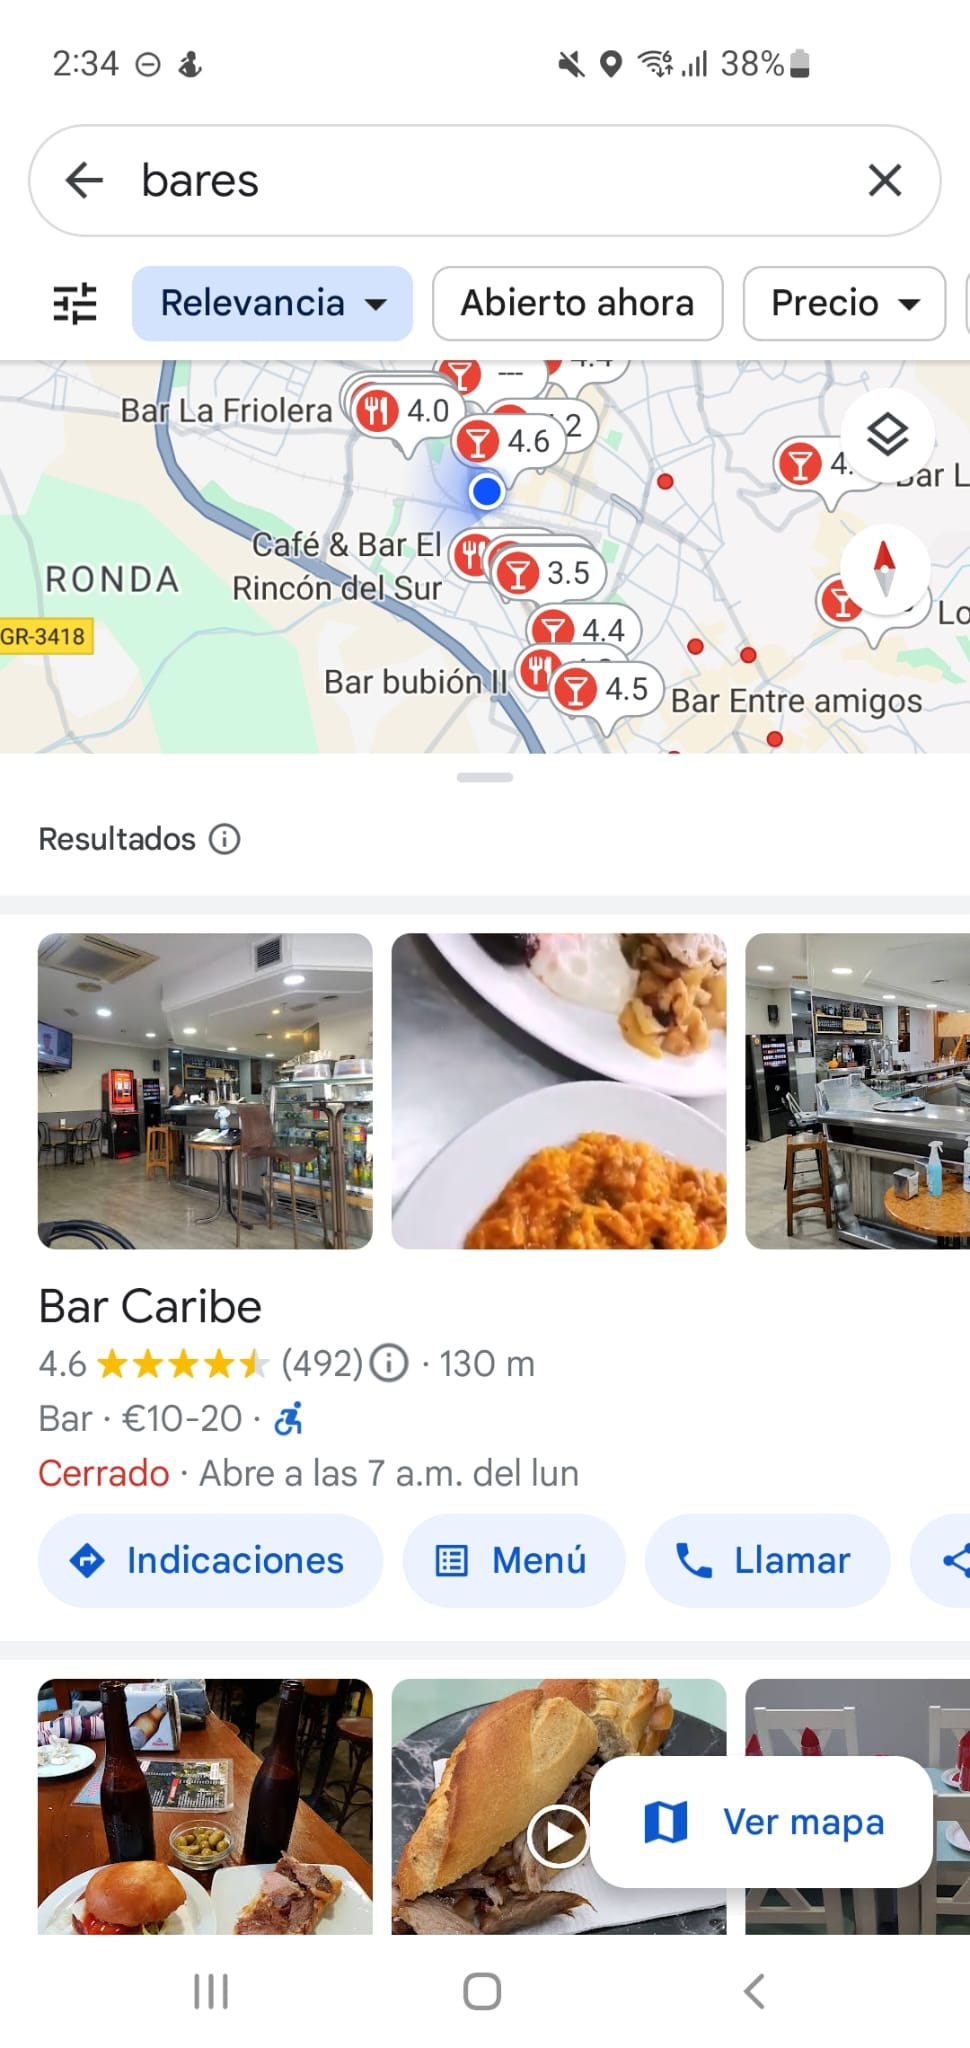
\includegraphics[width=\linewidth]{imagenes/GoogleMaps.jpeg}
        \caption{Google Maps}
        \label{fig:img1}
    \end{subfigure}%
    \hfill
    \begin{subfigure}{.3\textwidth}
        \centering
        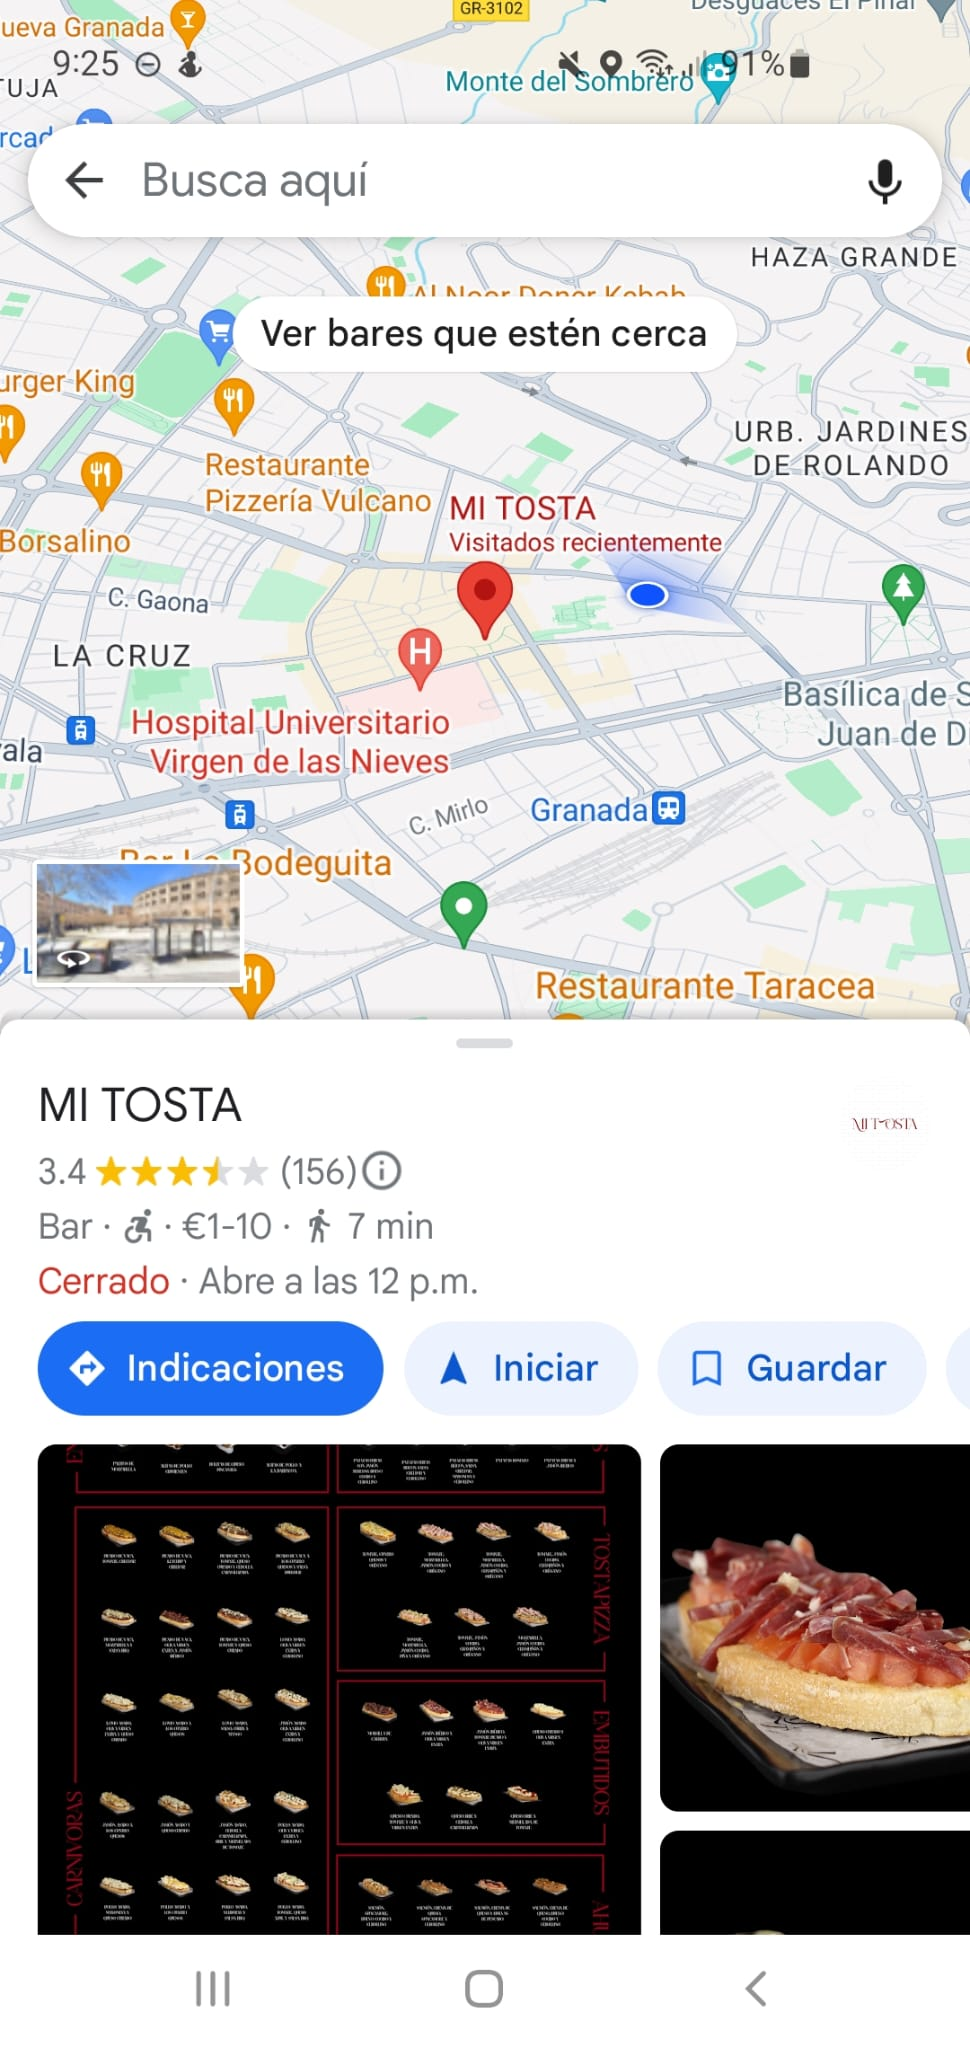
\includegraphics[width=\linewidth]{imagenes/Maps.jpeg}
        \caption{Google Maps}
        \label{fig:img2}
    \end{subfigure}%
    \hfill
    \begin{subfigure}{.3\textwidth}
        \centering
        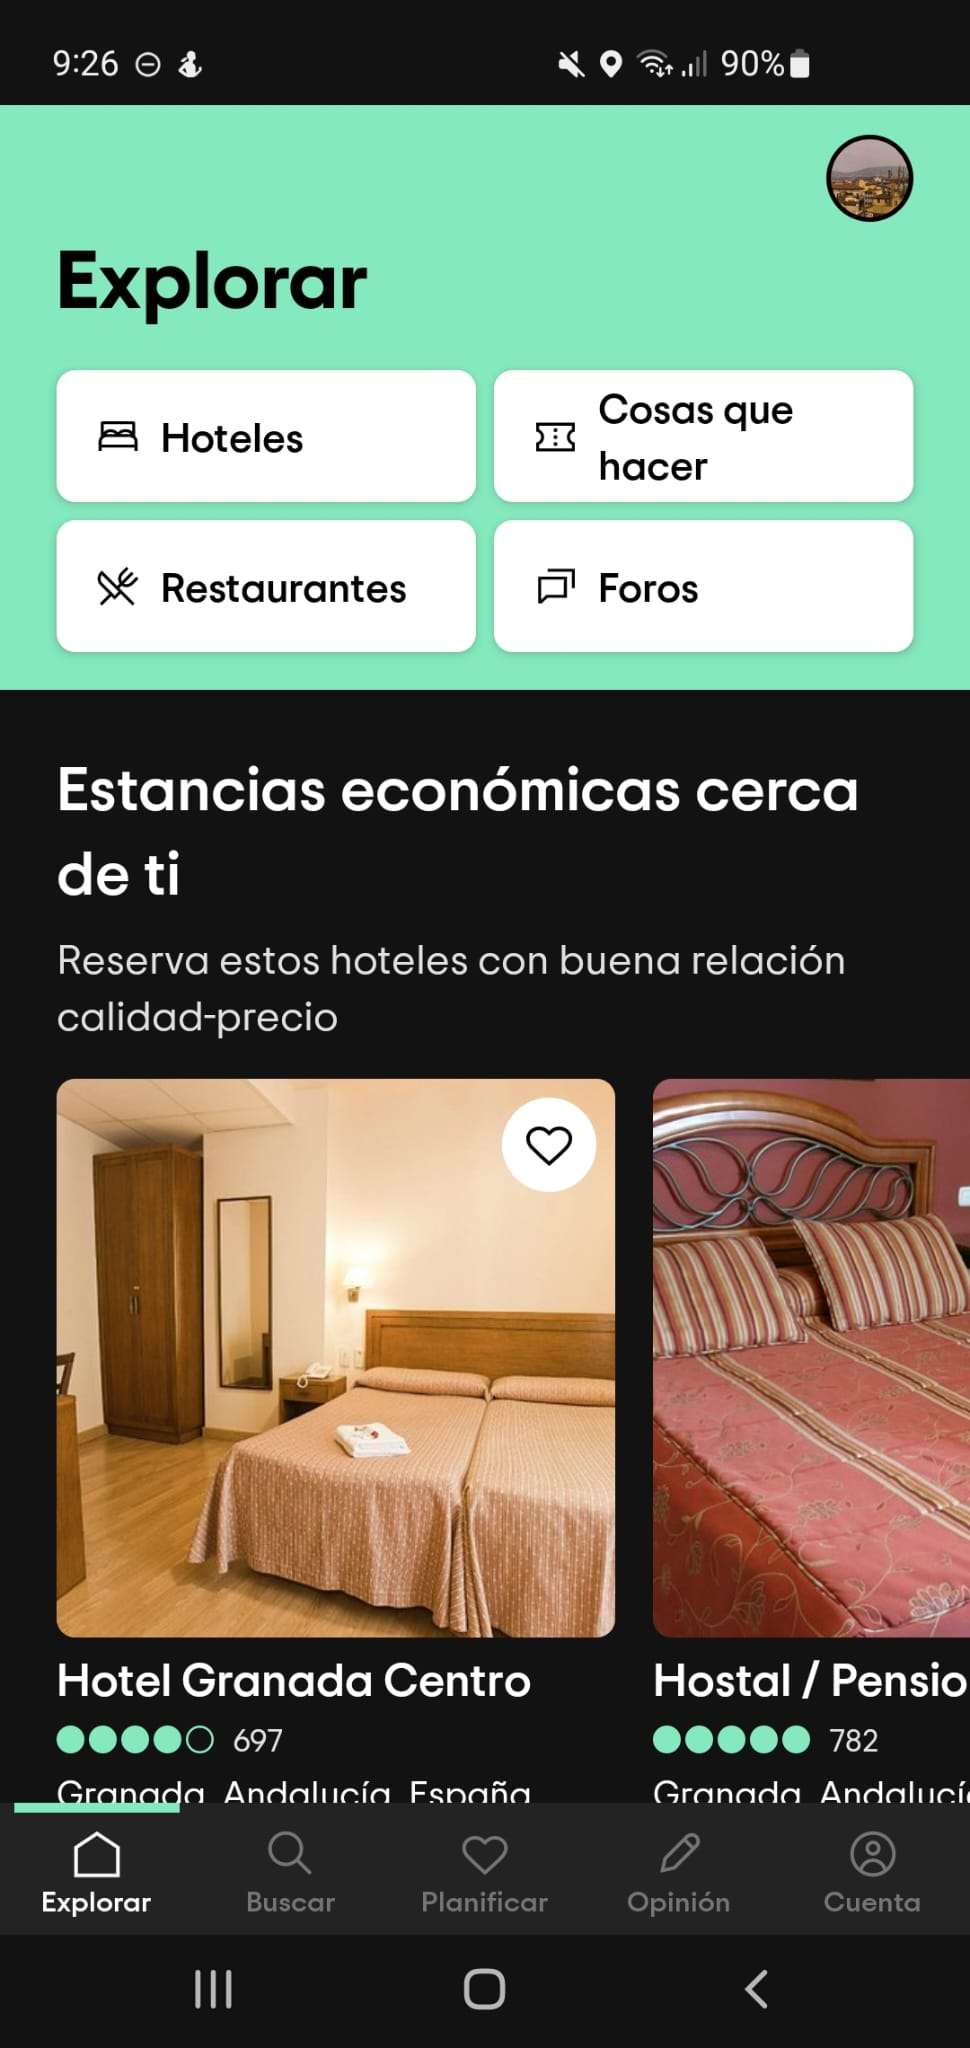
\includegraphics[width=\linewidth]{imagenes/TripAdvisor1.jpeg}
        \caption{TripAdvisor}
        \label{fig:img3}
    \end{subfigure}

    \vspace{1em}

    \begin{subfigure}{.3\textwidth}
        \centering
        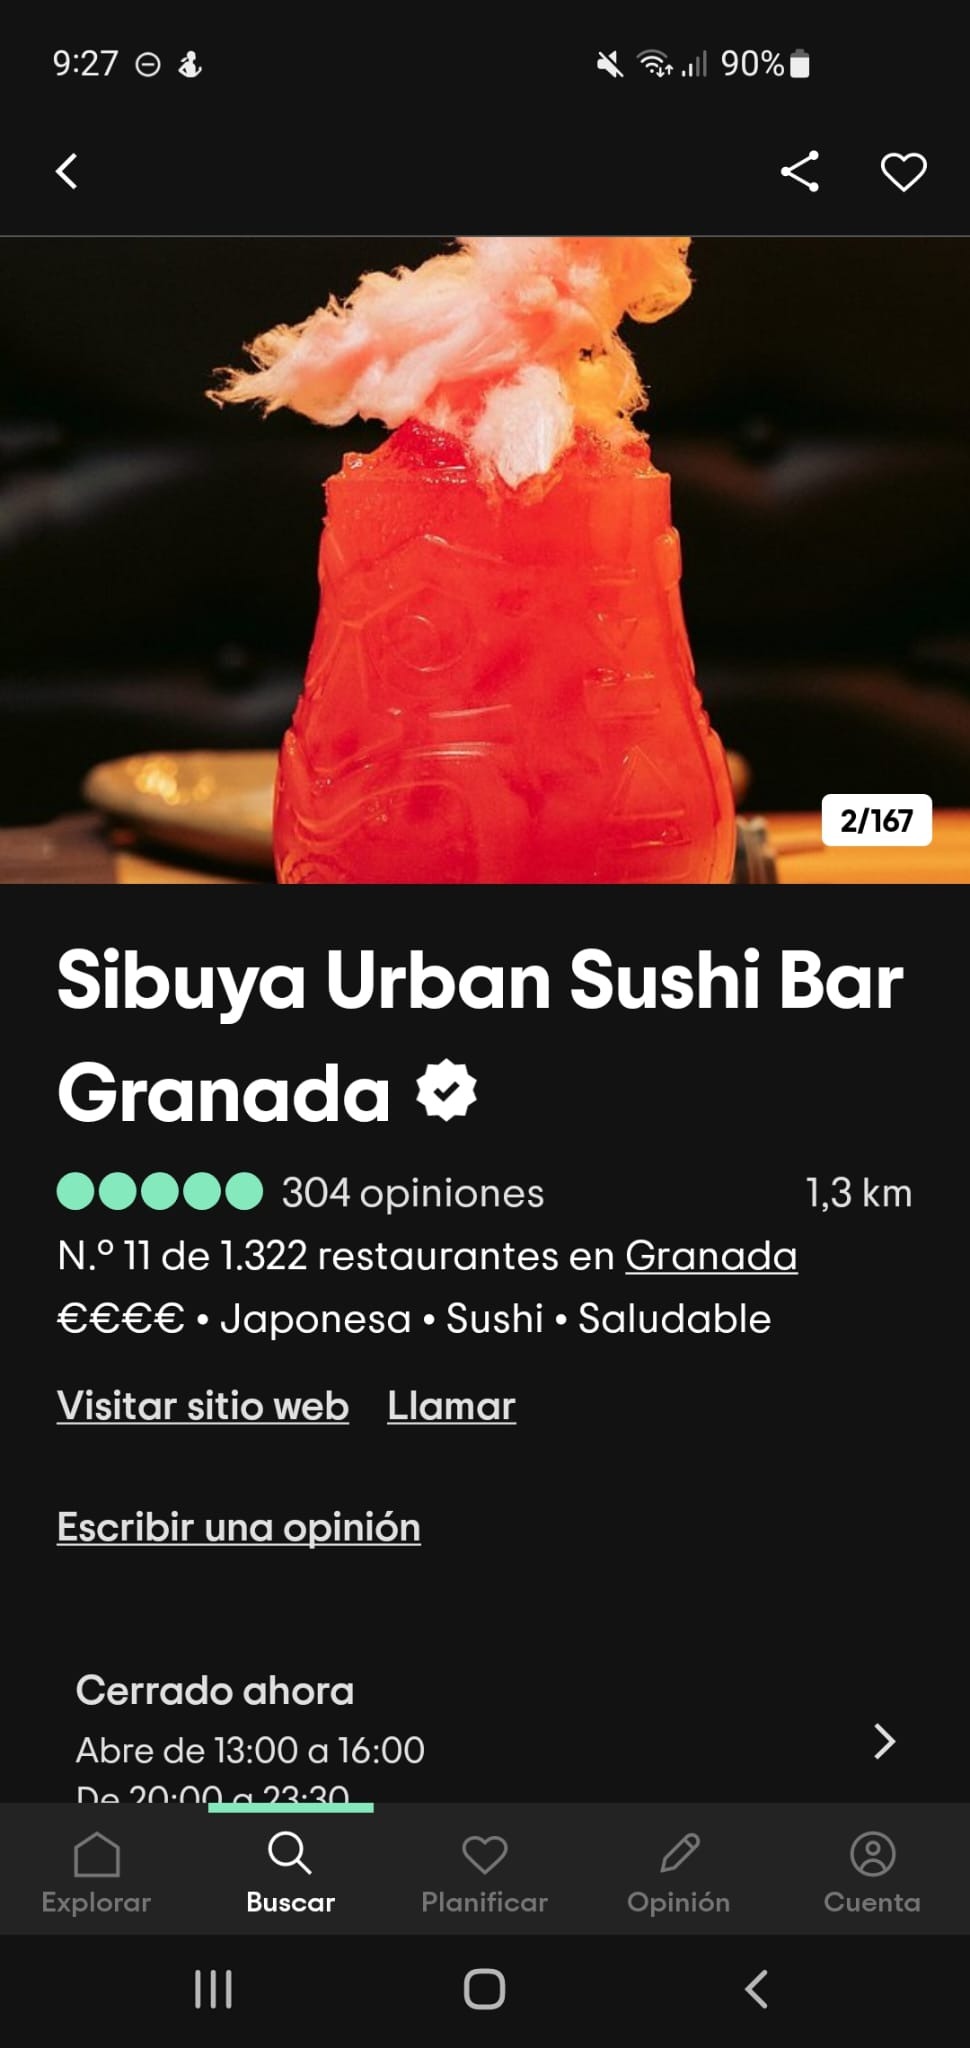
\includegraphics[width=\linewidth]{imagenes/TripAdvisor2.jpeg}
        \caption{TripAdvisor}
        \label{fig:img4}
    \end{subfigure}%
    \hfill
    \begin{subfigure}{.3\textwidth}
        \centering
        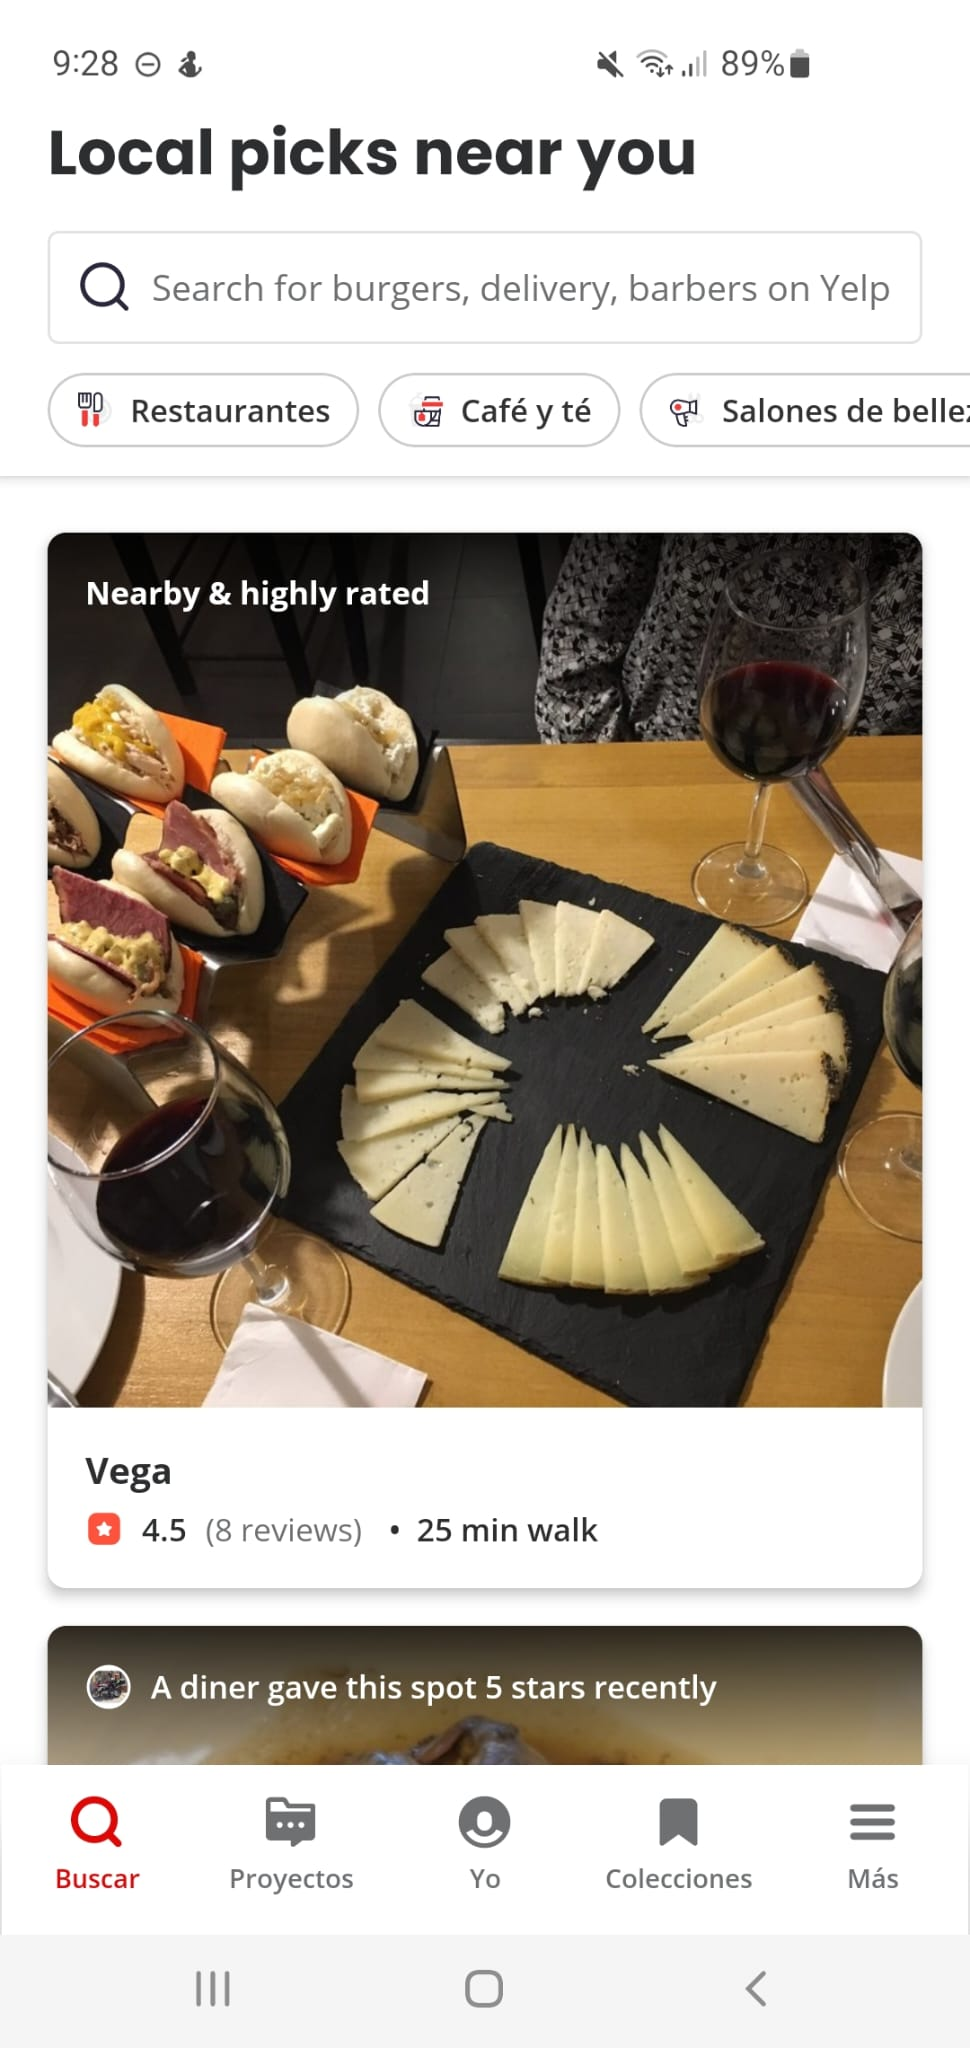
\includegraphics[width=\linewidth]{imagenes/Yelp1.jpeg}
        \caption{Yelp}
        \label{fig:img5}
    \end{subfigure}%
    \hfill
    \begin{subfigure}{.3\textwidth}
        \centering
        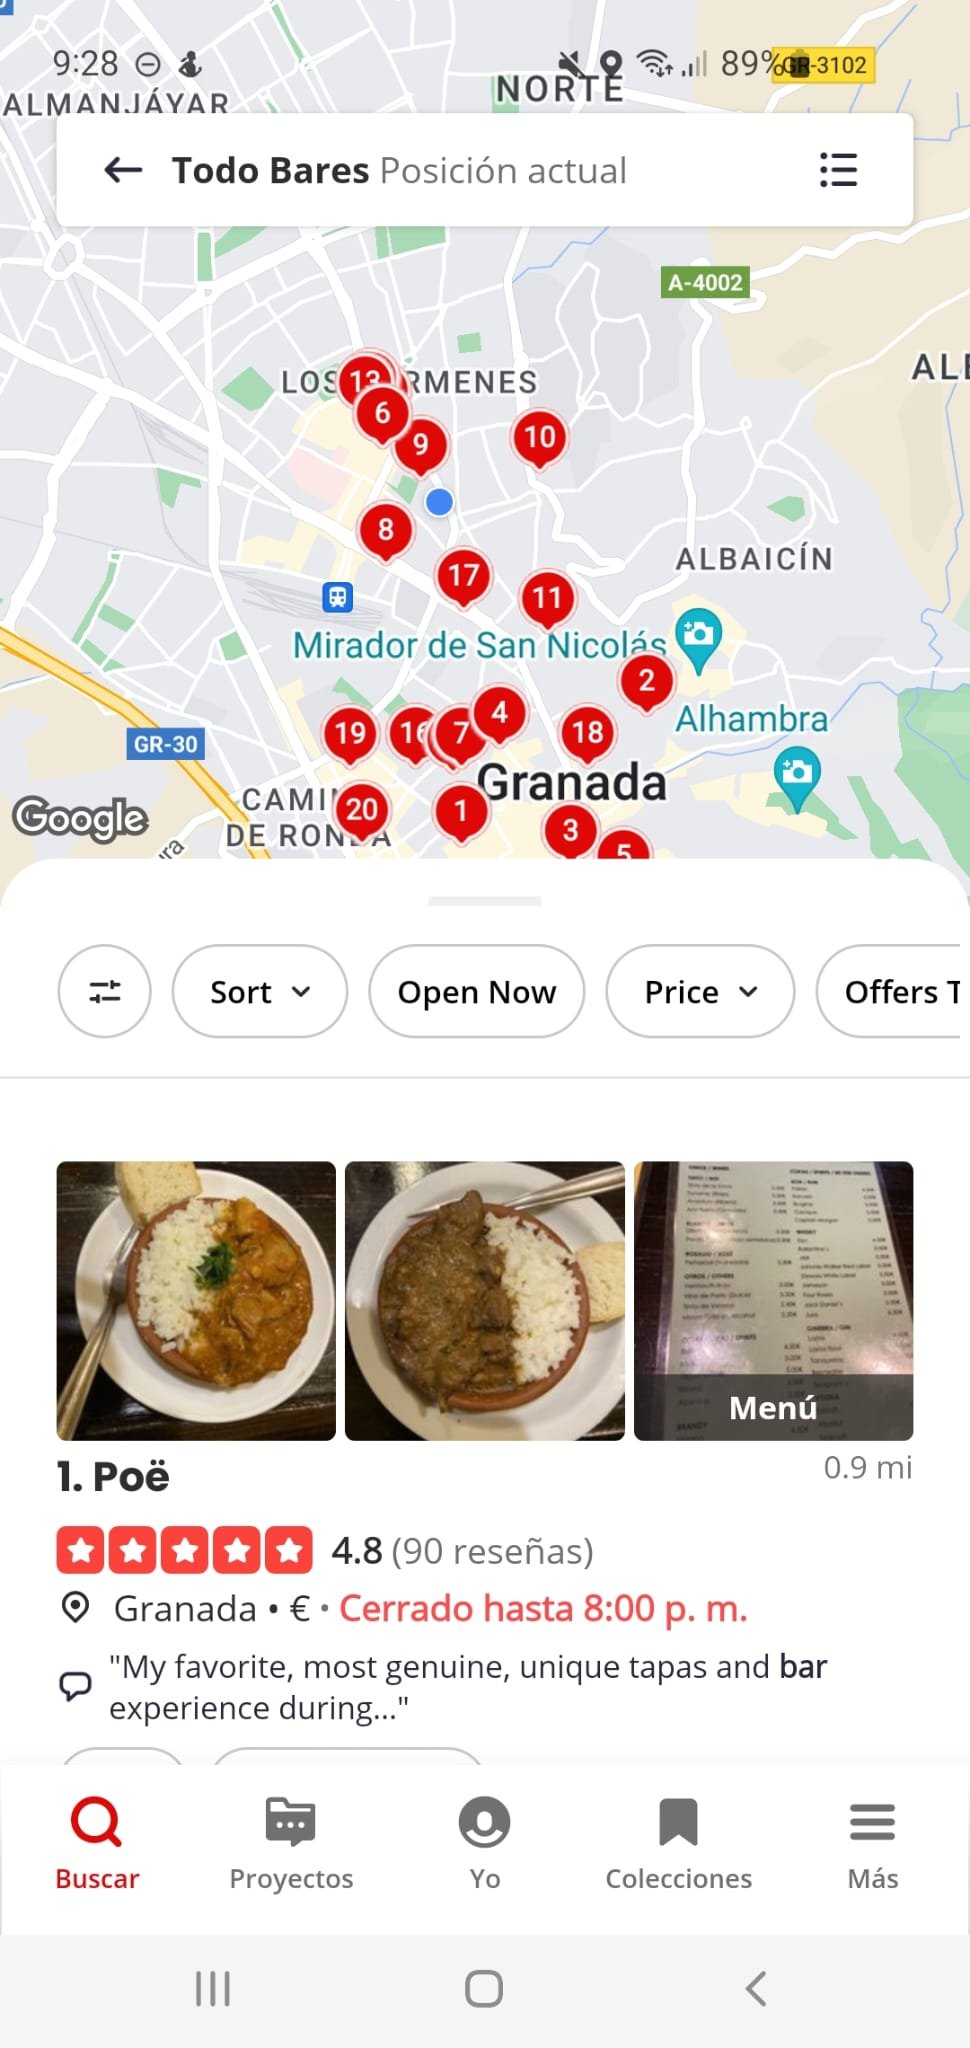
\includegraphics[width=\linewidth]{imagenes/Yelp2.jpeg}
        \caption{Yelp}
        \label{fig:img6}
    \end{subfigure}

    \caption{Comparación de aplicaciones orientadas al turismo}
    \label{fig:comparacion_apps}
\end{figure}

Estas aplicaciones aunque sean excelentes en muchos aspectos tienen ciertas limitaciones como pueden ser:

\begin{enumerate}

    \item \textbf{Información Fragmentada:} Los usuarios deben de consultar distintas plataformas y seguir a
          diversos establecimientos en sus redes sociales para estar al tanto de eventos u ofertas, lo que resulta en una
          experiencia fragmentada. Esta dispersión no es sólo ineficiente, sino que puede llevar a que los usuarios
          pierdan el interés y abandonen la búsqueda con consecuencia que pierdan una oportunidad importante de encontrar
          ese lugar que buscan.

    \item \textbf{Interacción Social Limitada:} Estas aplicaciones permiten leer reseñas y calificaciones en un
          establecimiento por parte de otros usuarios pero no permiten la creación de actividades entre amigos ni fomentan
          la organización y la interacción social.

    \item \textbf{Promoción y Gestión para Establecimientos:} La gestión de los perfiles y la promoción de eventos y
          ofertas en estas plataformas no es una prioridad. Estas aplicaciones tienden a centrarse más en la experiencia
          del usuario, ofreciendo calificaciones y reseñas de los establecimientos, pero no promueven activamente los
          lugares con los eventos y ofertas que pueden tener.

    \item \textbf{Enfoque Amplio y no Exclusivo al Ocio:} Estas aplicaciones abarcan un conjunto de funcionalidades
          no exclusivamente centradas en el ocio. Por ejemplo, TripAdvisor proporciona información sobre hoteles,
          atracciones turísticas y restaurantes, mientras que Google requiere búsquedas individuales de cada
          establecimiento hasta encontrar uno que se ajuste a las necesidades del usuario.

\end{enumerate}

\section{Soluciones HangOut}

Para solucionar estas limitaciones se ha desarrollado HangOut, una aplicación móvil diseñada para asistir a las personas para encontrar un establecimiento o evento adecuado a sus gustos que integra y mejora las funcionalidades existentes con características innovadoras:


\begin{enumerate}
    \item \textbf{Centralización de la Información:} HangOut centraliza la información de diversos establecimientos y eventos, permitiendo al usuario encontrar rápidamente opciones que se ajusten a sus preferencias sin necesidad de consultar múltiples fuentes.

    \item \textbf{Interacción y Organización Social:} La aplicación permite a los usuarios seguir a otros, crear actividades y organizar salidas grupales de manera más eficiente, eliminando la necesidad de coordinarse a través de múltiples aplicaciones de mensajería.

    \item \textbf{Herramientas para Administradores de Establecimiento:} HangOut proporciona a los administradores una plataforma para gestionar sus perfiles de establecimiento indicando el ambiente, eventos y ofertas, facilitando así la promoción y gestión de sus servicios de manera más eficaz.

    \item \textbf{Enfoque Exclusivo:} La aplicación se distingue por su enfoque exclusivo en el ocio y la eficiencia en la organización de eventos. Combinando la funcionalidad de creaciones de actividades en grupos específicos con la búsqueda de establecimientos y la personalización según las preferencias del usuario, ofreciendo una solución más específica para el ocio.
\end{enumerate}

\begin{table}[H]
    \centering
    \label{tab:comparison}
    \small
    \begin{tabularx}{\textwidth}{|X|X|X|X|X|X|}
        \hline
                                               & \textbf{TripAdvisor} & \textbf{Yelp} & \textbf{Google Maps} \\ \hline
        \textbf{Búsqueda por Filtros}          & Si                   & Si            & Si                   \\ \hline
        \textbf{Centralizado}                  & Si                   & Si            & Si                   \\ \hline
        \textbf{Exclusivo}                     & No                   & No            & No                   \\ \hline
        \textbf{Organización Social}           & No                   & No            & No                   \\ \hline
        \textbf{Promoción de Establecimientos} & Si                   & No            & No                   \\ \hline
    \end{tabularx}
    \caption{Comparación de características de aplicaciones para el turismo}

\end{table}




\chapter{Planificación}
\section{Metodología de Desarrollo Ágil}

Las metodologías ágiles de desarrollo de software son ampliamente utilizadas hoy en día debido a su alta flexibilidad y capacidad de adaptación. Estas metodologías permiten a los equipos de trabajo ser más productivos y eficientes, ya que tienen claridad sobre las tareas durante el desarrollo. En el proceso, el software se va adaptando a las nuevas necesidades y requerimientos que vayan surgiendo, facilitando la creación de aplicaciones funcionales. [REF]

Este tipo de metodologías de desarrollo tienen ciertas características claves que hace que destaque respecto a las tradicionales:

\begin{enumerate}
    \item \textbf{Flexibilidad y Agilidad:} Permiten la adaptación continua del software a medida que se identifican nuevas necesidades por parte de los usuarios.

    \item \textbf{Desarrollo Incremental:} En cada ciclo de desarrollo se van agregando nuevas funcionalidades.

    \item \textbf{Ciclos de Desarrollo Cortos:} Los ciclos de desarrollo, conocidos como iteraciones o sprints, son cortos y permiten la entrega continua de incremento funcionales del software, facilitando un feedback continuo.
\end{enumerate}

\subsection{Ejemplos de Metodologías}

\begin{enumerate}
    \item \textbf{Kanban:} Se basa en dividir las tareas en porciones más pequeñas y organizarlas en un tablero de trabajo con columnas de tareas pendientes, en curso y finalizadas. Este sistema crea un flujo de trabajo visual que ayuda a priorizar las tareas y mejorar el valor del producto.

    \item \textbf{Scrum:} Es una metodología incremental que organiza los requisitos y tareas en ciclos cortos y fijos, denominados sprints. Las etapas incluyen la planificación del sprint, ejecución, reuniones diarias y revisión de los resultados. Cada iteración completa estas etapas, permitiendo entregar un producto funcional al final de cada sprint.

    \item \textbf{Lean:} Enfocada en equipos pequeños y altamente capacitados, promueve la rápida ejecución de tareas y valora principalmente el compromiso y la capacidad de aprendizaje del equipo. Los ciclos cortos permiten adaptarse rápidamente a los cambios y mejorar el producto.
\end{enumerate}

Para llevar a cabo mi proyecto, decidí utilizar una metodología de desarrollo ágil como es \textbf{Scrum}. Esta elección fue motivada por diferentes razones con el objetivo de maximizar la eficiencia y calidad del producto final. Los principales motivos fueron:

\begin{enumerate}
    \item \textbf{Adaptación a Cambios Continuos:} Al desempeñar el rol de programador y usuario de la aplicación la capacidad de adaptación se volvió un papel muy importante, los requisitos podían cambiar a medida que avanzaba el desarrollo. Utilizando Scrum, con sus sprints cortos y revisiones frecuentes, me permitió ajustar el rumbo del proyecto ágilmente.

    \item \textbf{Desarrollo Incremental:} Me permitió dividir el trabajo en partes manejables y poder completar incrementos funcionales del software de manera continua. Cada sprint incluía la implementación y prueba de nuevas funcionalidades.

    \item \textbf{Mejora Continua:} Aunque trabajé de forma independiente, seguí prácticas de Scrum como revisiones de sprint para mantener la organización del proyecto. Adicionalmente, me reunía cada cierto tiempo con mi tutor para poder revisar mi avance.

\end{enumerate}


\section{Cronograma y Planificación}

El proyecto comenzó a mitad de febrero de 2024, con la meta de ser completado a finales de junio del mismo año. Para visualizar la planificación del mismo, se presenta un Diagrama de Gantt. Este diagrama es una representación gráfica del cronograma del proyecto, donde las tareas se describen en el  eje vertical y el tiempo empleado en cada una de ellas en el eje horizontal. El diagrama muestra las fechas de inicio y finalización del proyecto, facilitando el seguimiento y la gestión de las distintas etapas del desarrollo.

La aplicación se ha desarrollado utilizando tecnologías como Python y React Native, de las cuales no tenía experiencia previa. Por lo tanto, la planificación del proyecto se realizó teniendo en cuenta el tiempo necesario para aprender y familiarizarme con estos lenguajes. Este proceso incluyó la dedicación del tiempo adicional para la formación y la práctica de ambas tecnologías, asegurando así un desarrollo ágil y eficiente de la aplicación.

\subsection{Diagrama de Gantt}

\begin{figure}[H]
    \centering
    \scriptsize
    \resizebox{\textwidth}{!}{%
        \begin{ganttchart}[
                hgrid,
                vgrid={*{6}{draw=none}, dotted},
                title/.append style={fill=blue!10},
                title label font=\tiny,
                title height=1,
                bar/.append style={fill=gray!30},
                bar height=.4,
                y unit chart=0.7cm,
                x unit=0.2cm,
                time slot format=isodate,
                milestone left shift=-1,
                milestone right shift=2,
                group/.append style={font=\normalsize}
            ]{2024-02-16}{2024-06-24}

            \gantttitlecalendar{month=name} \\

            \ganttgroup[inline=false]{\textbf{\normalsize Investigación y Formación Inicial}}{2024-02-16}{2024-03-01} \\
            \ganttbar{Estudio de Python y Flask}{2024-02-16}{2024-02-24} \\
            \ganttbar{Estudio React Native}{2024-02-25}{2024-03-01} \\

            \ganttnewline

            \ganttgroup[inline=false]{\textbf{\normalsize Planificación del Proyecto}}{2024-03-01}{2024-03-09} \\

            \ganttnewline

            \ganttgroup[inline=false]{\textbf{\normalsize Requisitos del Proyecto}}{2024-03-09}{2024-03-17} \\
            \ganttbar{Requisitos Funcionales}{2024-03-09}{2024-03-14} \\
            \ganttbar{Requisitos No Funcionales}{2024-03-15}{2024-03-17} \\

            \ganttnewline

            \ganttgroup[inline=false]{\textbf{\normalsize Diseño del Sistema}}{2024-03-17}{2024-03-31} \\
            \ganttbar{Diseño de MockUps Iniciales}{2024-03-17}{2024-03-20} \\
            \ganttbar{Diseño de Base de Datos}{2024-03-21}{2024-03-24} \\
            \ganttbar{Elaboración de Diagramas UML}{2024-03-25}{2024-03-31} \\

            \ganttnewline

            \ganttgroup[inline=false]{\textbf{\normalsize Desarrollo del BackEnd}}{2024-04-01}{2024-04-30} \\
            \ganttbar{Configuración del Entorno de Desarrollo}{2024-04-01}{2024-04-03} \\
            \ganttbar{Implementación de Clases y Modelo}{2024-04-03}{2024-04-14} \\
            \ganttbar{Implementación de EndPoints API}{2024-04-15}{2024-04-27} \\
            \ganttbar{Pruebas de EndPoint con POSTMAN}{2024-04-28}{2024-04-30} \\

            \ganttnewline

            \ganttgroup[inline=false]{\textbf{\normalsize Desarrollo de FrontEnd}}{2024-05-01}{2024-06-06} \\
            \ganttbar{Diseño en Figma}{2024-05-01}{2024-05-04} \\
            \ganttbar{Configuración del Entorno FrontEnd}{2024-05-04}{2024-05-07} \\
            \ganttbar{Desarrollo de Pantallas y Componentes}{2024-05-08}{2024-05-17} \\
            \ganttbar{Pruebas de Visualización en ExpoGo}{2024-05-17}{2024-05-18} \\
            \ganttbar{Integración del FrontEnd con BackEnd}{2024-05-19}{2024-05-25} \\
            \ganttbar{Implementación de Navegación entre Pantallas}{2024-05-26}{2024-06-06} \\

            \ganttnewline

            \ganttgroup[inline=false]{\textbf{\normalsize Documentación del Proyecto}}{2024-06-06}{2024-06-24} \\

        \end{ganttchart}
    }
    \caption{Diagrama de Gantt detallado con la planificación y fases de desarrollo}
    \label{fig:gantt_diagram_detailed}
\end{figure}

\section{Recursos y Materiales}

En este apartado se analizan los recursos y materiales utilizados durante el transcurso del proyecto.

\subsection{Recursos Humanos}

Para el desarrollo de la aplicación, el principal y único recurso humano he sido yo, ya que he desempeñado los roles de desarrollador y usuario. Además, es importante mencionar a mi tutor, quien me ha guiado a lo largo del proceso, proporcionando orientación y apoyo.

\subsection{Materiales}

Para el desarrollo del proyecto se ha utilizado un portátil personal y un segundo monitor, lo cual ha sido de gran ayuda a la hora de programar, permitiendo una mayor eficiencia y comodidad en la gestión de múltiples ventanas y herramientas. A parte de los materiales utilizados para el desarrollo también se ha utillzado un smartphone para la prueba del frontend utilizando la aplicación Expo Go:

\begin{enumerate}
    \item \textbf{Portátil:} ASUS TUF F15 FX506HC - Portátil de 15.6" Full HD 144Hz (Intel Core i5-11400H, 16GB RAM, 512GB SSD, NVIDIA RTX 3050-4GB). Con valor actual de 699.99 \EUR{} [REF]

    \item \textbf{Monitor:} BenQ GW2480 - Monitor IPS LED de 23.8 Pulgadas 1080p. Con valor actual de 99.99 \EUR{} [REF]

    \item \textbf{Smartphone:} Samsung Galaxy S10e - Smartphone de 5.8”, Dual SIM, 128 GB. Con valor actual de 329.99 \EUR{} [REF]
\end{enumerate}

\section{Presupuesto}

En este apartado se analiza y se describen los costes del proyecto utilizando información proporcionada por las bases de cotización para contingencias comunes del año 2024, según la Seguridad Social de España. El perfil será el de un ingeniero informático junior y teniendo en cuenta que las bases de cotización oscilan entre un mínimo de 1.847,40 \EUR{} y un máximo de 4.720,50 €. Se asumirá el uso de la base mínima de cotización y la duración de 5 meses del proyecto. [REF]

Con esta información el coste total del salario para un ingeniero informático junior durante la duración del proyecto sería de
\[
    \textbf{Salario Informatico Junior} = 1\,847{,}40 \text{ \EUR{}/mes} \times 5 \text{ meses} = 9\,237 \text{\EUR{}}
\]


Si por su contraparte quisiéramos ver el coste total del salario para un ingeniero informático senior durante la duración del proyecto y utilizando el máximo de las bases de cotización mencionadas anteriormente, procederíamos de la siguiente manera:
\[
    \textbf{Salario Informatico Senior} = 4\,720{,}50 \text{ \EUR{}/mes} \times 5 \text{ meses} = 23\,602{,}50 \text{\EUR{}}
\]

Estas estimaciones no toman costes adicionales más allá de los descritos anteriormente.

En lo que respecta a las licencias para este proyecto, todas las tecnologías utilizadas han sido de código abierto con el fin de minimizar gastos. Como consecuencia a esta elección el coste total en licencias ha sido nulo.

Para estimar el coste del hardware mencionado en el apartado de materiales, es importante considerar la estimación de vida útil de un dispositivo, como puede ser un portátil o un smartphone, que es de 5 años.

\[
    \textbf{Coste Materiales} = 699{,}99 \text{ \EUR{}} + 329{,}99 \text{ \EUR{} } + 99{,}99 \text{ \EUR{}} = 1\,129{,}97 \text{ \EUR{}}
\]

\[
    \textbf{Coste Anual} = \frac{\text{Coste Material}}{5 \text{ años}} = 225{,}99 \text{ \EUR{}}
\]

\[
    \textbf{Coste Duración Proyecto} = \left( \frac{\text{Coste Anual}}{12 \text{ meses}} \right) \times 5 \text{ meses} = 94{,}16 \text{ \EUR{}}
\]

Sumando el coste del hardware al coste de los recursos humanos para un ingeniero informático junior, el coste total del proyecto durante estos 5 meses es de 9 331,16 \EUR{}. Para un ingeniero informático senior, el coste total del proyecto sería de 23 696,66 \EUR{}.



\chapter{Análisis}

A lo largo de esta sección se irán analizando los requisitos para el desarrollo del proyecto. La aplicación cubre la gestión de usuarios, administradores de establecimiento, establecimientos, actividades, eventos, ofertas y reseñas. Además, se describirán los requisitos no funcionales del sistema para garantizar una experiencia de usuario óptima y del correcto funcionamiento de la aplicación.

\section{Requisitos Funcionales}

Los requisitos funcionales son una parte esencial del desarrollo de sistemas, ya que capturan el comportamiento previo del sistema. Este comportamiento se puede expresar como servicios, tareas o funciones que el sistema debe realizar. Los requisitos funcionales se centran en lo que el sistema hará, describiendo el comportamiento del sistema en
términos de las acciones específicas que debe llevar a  cabo para cumplir con las necesidades y expectativas del usuario final. [REF]

A continuación se describirán los requisitos funcionales, divididos en apartados según su gestión principal. Esto permitirá una comprensión clara y detallada de los procesos y funcionalidades que la aplicación debe incluir para cumplir con sus objetivos y proporcionar una experiencia completa a sus usuarios.


\subsection{Gestión de Usuarios}

Este apartado describe las funcionalidades relativas a los usuarios. Al hablar de “Usuario” se referirá tanto a los usuarios genéricos del sistema como a un administrador de establecimiento. A continuación, se detallarán las funcionalidades para poder satisfacer las necesidades básicas de los usuarios:

\begin{table}[H]
    \centering
    \begin{tabular}{|c|p{10cm}|}
        \hline
        \multicolumn{2}{|c|}{\textbf{RF1 - Registro de Usuario}}                          \\
        \hline
        \textbf{Descripción}      & Permite a un nuevo usuario registrarse en el sistema. \\
        \hline
        \textbf{Datos de entrada} & Datos del usuario.                                    \\
        \hline
        \textbf{Datos de salida}  & Confirmación de registro exitoso.                     \\
        \hline
    \end{tabular}
    \caption{RF1 - Registro de Usuario}
\end{table}

\begin{table}[H]
    \centering
    \begin{tabular}{|c|p{10cm}|}
        \hline
        \multicolumn{2}{|c|}{\textbf{RF2 - Inicio de Sesión}}                                                                            \\
        \hline
        \textbf{Descripción}      & Permite a un usuario autenticarse e iniciar sesión en el sistema.                                    \\
        \hline
        \textbf{Datos de entrada} & Credenciales del usuario.                                                                            \\
        \hline
        \textbf{Datos de salida}  & Pantalla de inicio de usuario dependiendo si es usuario genérico o administrador de establecimiento. \\
        \hline
    \end{tabular}
    \caption{RF2 - Inicio de Sesión}
\end{table}

\begin{table}[H]
    \centering
    \begin{tabular}{|c|p{10cm}|}
        \hline
        \multicolumn{2}{|c|}{\textbf{RF3 - Consultar Usuario}}                                     \\
        \hline
        \textbf{Descripción}      & Permite ver la información del usuario que ha iniciado sesión. \\
        \hline
        \textbf{Datos de entrada} & Identificador del usuario.                                     \\
        \hline
        \textbf{Datos de salida}  & Datos del usuario.                                             \\
        \hline
    \end{tabular}
    \caption{RF3 - Consultar Usuario}
\end{table}

\begin{table}[H]
    \centering
    \begin{tabular}{|c|p{10cm}|}
        \hline
        \multicolumn{2}{|c|}{\textbf{RF4 - Modificar Usuario}}                                 \\
        \hline
        \textbf{Descripción}      & Permite actualizar los datos de un usuario en el sistema.  \\
        \hline
        \textbf{Datos de entrada} & Identificador del usuario, datos actualizados del usuario. \\
        \hline
        \textbf{Datos de salida}  & Confirmación de modificación exitosa.                      \\
        \hline
    \end{tabular}
    \caption{RF4 - Modificar Usuario}
\end{table}

\begin{table}[H]
    \centering
    \begin{tabular}{|c|p{10cm}|}
        \hline
        \multicolumn{2}{|c|}{\textbf{RF5 - Baja de Usuario}}                                               \\
        \hline
        \textbf{Descripción}      & Permite eliminar un usuario del sistema junto con sus datos asociados. \\
        \hline
        \textbf{Datos de entrada} & Identificador del usuario.                                             \\
        \hline
        \textbf{Datos de salida}  & Confirmación de baja exitosa.                                          \\
        \hline
    \end{tabular}
    \caption{RF5 - Baja de Usuario}
\end{table}

\begin{table}[H]
    \centering
    \begin{tabular}{|c|p{10cm}|}
        \hline
        \multicolumn{2}{|c|}{\textbf{RF6 - Seguir a Usuario}}                                                                     \\
        \hline
        \textbf{Descripción}      & Permite a un usuario seguir a otro usuario en el sistema, añadiéndolo a su lista de seguidos. \\
        \hline
        \textbf{Datos de entrada} & Identificador del usuario a seguir.                                                           \\
        \hline
        \textbf{Datos de salida}  & Confirmación de seguimiento de usuario, actualización de la lista de seguidos.                \\
        \hline
    \end{tabular}
    \caption{RF6 - Seguir a Usuario}
\end{table}

\begin{table}[H]
    \centering
    \begin{tabular}{|c|p{10cm}|}
        \hline
        \multicolumn{2}{|c|}{\textbf{RF7 - Dejar de Seguir a Usuario}}                                                                       \\
        \hline
        \textbf{Descripción}      & Permite a un usuario dejar de seguir a otro usuario en el sistema, eliminándolo de su lista de seguidos. \\
        \hline
        \textbf{Datos de entrada} & Identificador del usuario a dejar de seguir.                                                             \\
        \hline
        \textbf{Datos de salida}  & Confirmación de que se ha dejado de seguir a usuario, actualización de su lista de seguidos.             \\
        \hline
    \end{tabular}
    \caption{RF7 - Dejar de Seguir a Usuario}
\end{table}

\subsection{Gestión de Establecimientos}

Este apartado describe las funcionalidades relativas a los establecimientos, es decir, qué se puede hacer con ellos. A continuación, se detallarán las principales características y acciones disponibles para la gestión de los establecimientos dentro de la aplicación:

\begin{table}[H]
    \centering
    \begin{tabular}{|c|p{10cm}|}
        \hline
        \multicolumn{2}{|c|}{\textbf{RF8 - Crear Establecimiento}}                                                                                    \\
        \hline
        \textbf{Descripción}      & Permite a un administrador crear un nuevo establecimiento.                                                        \\
        \hline
        \textbf{Datos de entrada} & Datos del establecimiento.                                                                                        \\
        \hline
        \textbf{Datos de salida}  & Confirmación de la creación del establecimiento, actualización de la lista de establecimientos del administrador. \\
        \hline
    \end{tabular}
    \caption{RF8 - Crear Establecimiento}
\end{table}

\begin{table}[H]
    \centering
    \begin{tabular}{|c|p{10cm}|}
        \hline
        \multicolumn{2}{|c|}{\textbf{RF9 - Modificar Establecimiento}}                                         \\
        \hline
        \textbf{Descripción}      & Permite a un administrador actualizar los datos de un establecimiento.     \\
        \hline
        \textbf{Datos de entrada} & Identificador del establecimiento, datos actualizados del establecimiento. \\
        \hline
        \textbf{Datos de salida}  & Confirmación de modificación exitosa.                                      \\
        \hline
    \end{tabular}
    \caption{RF9 - Modificar Establecimiento}
\end{table}

\begin{table}[H]
    \centering
    \begin{tabular}{|c|p{10cm}|}
        \hline
        \multicolumn{2}{|c|}{\textbf{RF10 - Consultar Establecimiento}}                                                           \\
        \hline
        \textbf{Descripción}      & Permite a un usuario o administrador consultar los datos de un establecimiento en específico. \\
        \hline
        \textbf{Datos de entrada} & Identificador del establecimiento.                                                            \\
        \hline
        \textbf{Datos de salida}  & Datos del establecimiento.                                                                    \\
        \hline
    \end{tabular}
    \caption{RF10 - Consultar Establecimiento}
\end{table}

\begin{table}[H]
    \centering
    \begin{tabular}{|c|p{10cm}|}
        \hline
        \multicolumn{2}{|c|}{\textbf{RF11 - Eliminar Establecimiento}}                                                \\
        \hline
        \textbf{Descripción}      & Permite a un administrador eliminar un establecimiento.                           \\
        \hline
        \textbf{Datos de entrada} & Identificador del establecimiento.                                                \\
        \hline
        \textbf{Datos de salida}  & Confirmación de eliminación exitosa, actualización de la lista del administrador. \\
        \hline
    \end{tabular}
    \caption{RF11 - Eliminar Establecimiento}
\end{table}

\begin{table}[H]
    \centering
    \begin{tabular}{|c|p{10cm}|}
        \hline
        \multicolumn{2}{|c|}{\textbf{RF12 - Filtrar Establecimientos}}                                                        \\
        \hline
        \textbf{Descripción}      & Permite a un usuario poder filtrar los establecimientos según las preferencias indicadas. \\
        \hline
        \textbf{Datos de entrada} & Filtro aplicado.                                                                          \\
        \hline
        \textbf{Datos de salida}  & Establecimientos que cumplan con el filtro.                                               \\
        \hline
    \end{tabular}
    \caption{RF12 - Filtrar Establecimiento}
\end{table}

\subsection{Gestión de Eventos}

Este apartado describe la gestión de los eventos asociados a un establecimiento específico. Los eventos son importantes porque permiten a los establecimientos promocionar sus servicios, ayudando a los usuarios a decidir cuál se ajusta según sus necesidades. A continuación, se detallarán las principales acciones disponibles para la gestión de eventos:

\begin{table}[H]
    \centering
    \begin{tabular}{|c|p{10cm}|}
        \hline
        \multicolumn{2}{|c|}{\textbf{RF13 - Crear Evento}}                                                                                                       \\
        \hline
        \textbf{Descripción}      & Permite a un administrador crear un nuevo evento asociado a un establecimiento.                                              \\
        \hline
        \textbf{Datos de entrada} & Datos del evento                                                                                                             \\
        \hline
        \textbf{Datos de salida}  & Confirmación de creación del evento, actualización de la lista eventos del establecimiento en el cual se ha creado el evento \\
        \hline
    \end{tabular}
    \caption{RF13 - Crear Evento}
\end{table}

\begin{table}[H]
    \centering
    \begin{tabular}{|c|p{10cm}|}
        \hline
        \multicolumn{2}{|c|}{\textbf{RF14 - Modificar Evento}}                                                         \\
        \hline
        \textbf{Descripción}      & Permite a un administrador de establecimiento modificar un nuevo evento existente. \\
        \hline
        \textbf{Datos de entrada} & Identificador del evento, datos actualizados del evento.                           \\
        \hline
        \textbf{Datos de salida}  & Confirmación de modificación exitosa.                                              \\
        \hline
    \end{tabular}
    \caption{RF14 - Modificar Evento}
\end{table}

\begin{table}[H]
    \centering
    \begin{tabular}{|c|p{10cm}|}
        \hline
        \multicolumn{2}{|c|}{\textbf{RF15 - Consultar Evento}}                                                     \\
        \hline
        \textbf{Descripción}      & Permite a un usuario o administrador ver los datos de un evento en específico. \\
        \hline
        \textbf{Datos de entrada} & Identificador del evento.                                                      \\
        \hline
        \textbf{Datos de salida}  & Datos del evento.                                                              \\
        \hline
    \end{tabular}
    \caption{RF15 - Consultar Evento}
\end{table}

\begin{table}[H]
    \centering
    \begin{tabular}{|c|p{10cm}|}
        \hline
        \multicolumn{2}{|c|}{\textbf{RF16 - Eliminar Evento}}                                                                                              \\
        \hline
        \textbf{Descripción}      & Permite a un administrador eliminar un evento existente.                                                               \\
        \hline
        \textbf{Datos de entrada} & Identificador del evento.                                                                                              \\
        \hline
        \textbf{Datos de salida}  & Confirmación de eliminación exitosa, actualización de la lista de eventos del establecimiento que contenía ese evento. \\
        \hline
    \end{tabular}
    \caption{RF16 - Eliminar Evento}
\end{table}

\subsection{Gestión de Ofertas}

Este apartado describe la gestión de las ofertas asociadas a un establecimiento específico. Las ofertas son importantes porque permiten a los establecimientos promocionar sus servicios, ayudando a los usuarios a decidir cuál les conviene más entre los disponibles. A  continuación, se detallarán las principales acciones disponibles para la gestión de ofertas:

\begin{table}[H]
    \centering
    \begin{tabular}{|c|p{10cm}|}
        \hline
        \multicolumn{2}{|c|}{\textbf{RF17 - Crear Oferta}}                                                                                                         \\
        \hline
        \textbf{Descripción}      & Permiet a un administrador crear una nueva oferta asociada a un establecimiento.                                               \\
        \hline
        \textbf{Datos de entrada} & Datos de la oferta.                                                                                                            \\
        \hline
        \textbf{Datos de salida}  & Confirmación de creación exitosa, actualizacion de la lista de ofertas del establecimiento en el cual se ha creado esa oferta. \\
        \hline
    \end{tabular}
    \caption{RF17 - Crear Oferta}
\end{table}

\begin{table}[H]
    \centering
    \begin{tabular}{|c|p{10cm}|}
        \hline
        \multicolumn{2}{|c|}{\textbf{RF18 - Modificar Oferta}}                                   \\
        \hline
        \textbf{Descripción}      & Permite a un administrador modificar una oferta existente.   \\
        \hline
        \textbf{Datos de entrada} & Identificador de la oferta, datos actualizados de la oferta. \\
        \hline
        \textbf{Datos de salida}  & Confirmación de modificación exitosa.                        \\
        \hline
    \end{tabular}
    \caption{RF18 - Modificar Oferta}
\end{table}

\begin{table}[H]
    \centering
    \begin{tabular}{|c|p{10cm}|}
        \hline
        \multicolumn{2}{|c|}{\textbf{RF19 - Consultar Oferta}}                                                      \\
        \hline
        \textbf{Descripción}      & Permite a un usuario o administrador ver los datos de una oferta en específica. \\
        \hline
        \textbf{Datos de entrada} & Identificador de la oferta.                                                     \\
        \hline
        \textbf{Datos de salida}  & Datos de la oferta.                                                             \\
        \hline
    \end{tabular}
    \caption{RF19 - Consultar Oferta}
\end{table}

\begin{table}[H]
    \centering
    \begin{tabular}{|c|p{10cm}|}
        \hline
        \multicolumn{2}{|c|}{\textbf{RF20 - Eliminar Oferta}}                                                                                              \\
        \hline
        \textbf{Descripción}      & Permite a un administrador eliminar una oferta existente.                                                              \\
        \hline
        \textbf{Datos de entrada} & Identificador de la oferta.                                                                                            \\
        \hline
        \textbf{Datos de salida}  & Confirmación de eliminación exitosa, actualización de la lista de ofertas del establecimiento que contenía esa oferta. \\
        \hline
    \end{tabular}
    \caption{RF20 - Eliminar Oferta}
\end{table}

\subsection{Gestión de Actividades}

Este apartado describe la gestión de las actividades creadas por los usuarios para su grupo social cercano, con el fin de organizar y planificar salidas. A continuación, se detallan las principales acciones disponibles para la gestión de actividades:

\begin{table}[H]
    \centering
    \begin{tabular}{|c|p{10cm}|}
        \hline
        \multicolumn{2}{|c|}{\textbf{RF21 - Crear Actividad}}                                                                               \\
        \hline
        \textbf{Descripción}      & Permite a un usuario crear una nueva actividad.                                                         \\
        \hline
        \textbf{Datos de entrada} & Datos de la actividad.                                                                                  \\
        \hline
        \textbf{Datos de salida}  & Confirmación de creación de la actividad, actualización de la lista de actividades creadas del usuario. \\
        \hline
    \end{tabular}
    \caption{RF21 - Crear Actividad}
\end{table}

\begin{table}[H]
    \centering
    \begin{tabular}{|c|p{10cm}|}
        \hline
        \multicolumn{2}{|c|}{\textbf{RF22 - Modificar Actividad}}                                      \\
        \hline
        \textbf{Descripción}      & Permite a un usuario modificar una actividad creada.               \\
        \hline
        \textbf{Datos de entrada} & Identificador de la actividad, datos actualizados de la actividad. \\
        \hline
        \textbf{Datos de salida}  & Confirmación de modificación exitosa.                              \\
        \hline
    \end{tabular}
    \caption{RF2 - Modificar Actividad}
\end{table}

\begin{table}[H]
    \centering
    \begin{tabular}{|c|p{10cm}|}
        \hline
        \multicolumn{2}{|c|}{\textbf{RF23 - Consultar Actividad}}                                                              \\
        \hline
        \textbf{Descripción}      & Permite a un usuario poder consultar los datos de una actividad en la cual este participe. \\
        \hline
        \textbf{Datos de entrada} & Identificador de la actividad.                                                             \\
        \hline
        \textbf{Datos de salida}  & Datos de la actividad.                                                                     \\
        \hline
    \end{tabular}
    \caption{RF23 - Consultar Actividad}
\end{table}

\begin{table}[H]
    \centering
    \begin{tabular}{|c|p{10cm}|}
        \hline
        \multicolumn{2}{|c|}{\textbf{RF24 - Eliminar Actividad}}                                                                       \\
        \hline
        \textbf{Descripción}      & Permite a un usuario eliminar una actividad creada.                                                \\
        \hline
        \textbf{Datos de entrada} & Identificador de la actividad.                                                                     \\
        \hline
        \textbf{Datos de salida}  & Confirmación de eliminación exitosa, actualización de la lista de actividades creadas del usuario. \\
        \hline
    \end{tabular}
    \caption{RF24 - Eliminar Actividad}
\end{table}

\begin{table}[H]
    \centering
    \begin{tabular}{|c|p{10cm}|}
        \hline
        \multicolumn{2}{|c|}{\textbf{RF25 - Invitar Usuario a Actividad}}                                                                                   \\
        \hline
        \textbf{Descripción}      & Permite a un usuario invitar a otros usuarios a participar en una actividad.                                            \\
        \hline
        \textbf{Datos de entrada} & Identificador del usuario a invitar.                                                                                    \\
        \hline
        \textbf{Datos de salida}  & Confirmación de adición de un nuevo usuario a la actividad, actualización de la lista de participantes de la actividad. \\
        \hline
    \end{tabular}
    \caption{RF25 - Invitar Usuario a Actividad}
\end{table}

\subsection{Gestión de Reseñas}

Este apartado describe la gestión de las reseñas a un establecimiento. Las reseñas son cruciales para mostrar a los usuarios los establecimientos según las evaluaciones y comentarios de otros clientes. Además, son importantes para los administradores de establecimientos, ya que pueden utilizar el feedback para mejorar sus servicios. A continuación, se detallan las principales acciones para la gestión de las reseñas:

\begin{table}[H]
    \centering
    \begin{tabular}{|c|p{10cm}|}
        \hline
        \multicolumn{2}{|c|}{\textbf{RF26 - Crear Reseña}}                                                                                                                                                 \\
        \hline
        \textbf{Descripción}      & Permite a un usuario dejar reseñas a un establecimiento.                                                                                                               \\
        \hline
        \textbf{Datos de entrada} & dentificador del establecimiento, datos de la reseña.                                                                                                                  \\
        \hline
        \textbf{Datos de salida}  & Confirmación de que la reseña ha sido publicada, actualización de la lista de reseñas del establecimiento, actualización de las listas de reseñas creadas del usuario. \\
        \hline
    \end{tabular}
    \caption{RF26 - Crear Reseña}
\end{table}

\begin{table}[H]
    \centering
    \begin{tabular}{|c|p{10cm}|}
        \hline
        \multicolumn{2}{|c|}{\textbf{RF27 - Consultar Reseña}}                                                             \\
        \hline
        \textbf{Descripción}      & Permite a un usuario o administrador ver las reseñas de un establecimiento específico. \\
        \hline
        \textbf{Datos de entrada} & Identificador del establecimiento.                                                     \\
        \hline
        \textbf{Datos de salida}  & Reseñas del establecimiento.                                                           \\
        \hline
    \end{tabular}
    \caption{RF27 - Consultar Reseña}
\end{table}

\section{Requisitos No Funcionales}

Los requisitos no funcionales son aquellos que especifican los criterios que pueden ser utilizados para juzgar el funcionamiento de un sistema, en lugar de describir los comportamientos específicos. A diferencia de los requisitos funcionales, que detallan lo que el sistema debe hacer, los requisitos no funcionales definen cómo debe ser el sistema en términos de calidad y restricciones operativas, asegurando que el sistema cumpla con los estándares de calidad esperados. [REF]

\begin{table}[H]
    \centering
    \begin{tabular}{|c|p{10cm}|}
        \hline
        \multicolumn{2}{|c|}{\textbf{RNF1 - Usabilidad}}                                       \\
        \hline
        \textbf{Descripción} & La aplicación será intuitiva y fácil de usar para los usuarios. \\
        \hline
        \textbf{Criterios}   & Interfaz de usuario sencilla e intuitiva.                       \\
        \hline
    \end{tabular}
    \caption{RNF1 - Usabilidad}
\end{table}

\begin{table}[H]
    \centering
    \begin{tabular}{|c|p{10cm}|}
        \hline
        \multicolumn{2}{|c|}{\textbf{RNF2 - Rendimiento}}                                             \\
        \hline
        \textbf{Descripción} & La aplicación deberá responder rápidamente a las consultas realizadas. \\
        \hline
        \textbf{Criterios}   & Tiempos de respuestas rápidos para las peticiones realizadas.          \\
        \hline
    \end{tabular}
    \caption{RNF2 - Rendimiento}
\end{table}

\begin{table}[H]
    \centering
    \begin{tabular}{|c|p{10cm}|}
        \hline
        \multicolumn{2}{|c|}{\textbf{RNF3 - Seguridad}}                                                                              \\
        \hline
        \textbf{Descripción} & La aplicación protegerá la información sensible relacionada con los datos personales de los usuarios. \\
        \hline
        \textbf{Criterios}   & Los datos sensibles de los usuarios solo podrán ser consultados por ellos mismos.                     \\
        \hline
    \end{tabular}
    \caption{RNF3 - Seguridad}
\end{table}

\begin{table}[H]
    \centering
    \begin{tabular}{|c|p{10cm}|}
        \hline
        \multicolumn{2}{|c|}{\textbf{RNF4 - Compatibilidad}}                                                                                                 \\
        \hline
        \textbf{Descripción} & La aplicación funcionará correctamente independientemente del dispositivo móvil utilizado siempre y cuando sea un smartphone. \\
        \hline
        \textbf{Criterios}   & El diseño del frontend en React Native permite poder desplegar el archivo APK para Android y el archivo para iOS.             \\
        \hline
    \end{tabular}
    \caption{RNF4 - Compatibilidad}
\end{table}

\begin{table}[H]
    \centering
    \begin{tabular}{|c|p{10cm}|}
        \hline
        \multicolumn{2}{|c|}{\textbf{RNF5 - Escalabilidad}}                                                                                  \\
        \hline
        \textbf{Descripción} & La aplicación debe ser capaz de escalar y manejar el aumento de la carga manteniendo el nivel de rendimiento. \\
        \hline
        \textbf{Criterios}   & El sistema permite el crecimiento de carga según aumente el número de usuarios gracias a su arquitectura.     \\
        \hline
    \end{tabular}
    \caption{RNF5 - Escalabilidad}
\end{table}

\begin{table}[H]
    \centering
    \begin{tabular}{|c|p{10cm}|}
        \hline
        \multicolumn{2}{|c|}{\textbf{RNF6 - Mantenibilidad}}                                                                                                                                                     \\
        \hline
        \textbf{Descripción} & La aplicación debe poder proveer actualizaciones y mantenimiento regulable para su continuo desarrollo.                                                                           \\
        \hline
        \textbf{Criterios}   & La documentación se realizará de una forma clara permitiendo el entendimiento del código y podiendo realizar actualizaciones para el beneficio de la experiencia de los usuarios. \\
        \hline
    \end{tabular}
    \caption{RNF6 - Mantenibilidad}
\end{table}

\section{Modelos de Caso de Uso}

Los modelos de caso de uso son representaciones gráficas que describen cómo los usuarios interactúan con el sistema para lograr un objetivo específico. Estos modelos se utilizan para capturar y definir los requisitos funcionales del sistema., identificando las diferentes formas en que los usuarios pueden utilizar el sistema y las respuestas del sistema a estas interacciones. Los modelos de casos de uso ayudan a comunicar claramente las funcionalidades esperadas del sistema a todas las partes interesadas, asegurando que todos tengan una comprensión común de los requerimientos. [REF]

\subsection{Actores del Sistema}

La interacción de la aplicación se basa en dos tipos de actores: usuarios genéricos y administradores de establecimiento. Es importante destacar que el acceso a la aplicación está restringida a usuarios registrados, ya que se busca asegurar que cada interacción dentro del sistema se realice de una manera personalizada.

\begin{enumerate}
    \item \textbf{Usuario Genérico:} Los usuarios genéricos son los clientes de la aplicación, aquellos para los cuales está destinado su uso. Pueden consultar establecimientos según las preferencias indicadas, ver las ofertas y eventos disponibles, y crear actividades sociales. Estas funcionalidades permiten a los usuarios personalizar su experiencia y aprovechar al máximo los servicios ofrecidos por la aplicación.

    \item \textbf{Administrador de Establecimiento:} Los administradores de establecimientos interactúan con la aplicación para la creación, administración y promoción de sus establecimientos. Esto incluye la creación de ofertas y eventos, así como la gestión general de la información del establecimiento. Estas funcionalidades permiten a los administradores optimizar la visibilidad y el atractivo de sus establecimientos dentro de la aplicación.
\end{enumerate}

\subsection{Escenarios de Casos de Uso}

\begin{table}[h]
    \centering
    \begin{tabular}{|c|p{10cm}|}
        \hline
        \multicolumn{2}{|c|}{\textbf{CU1 - Registrar Usuario}}                               \\
        \hline
        \textbf{Actores}         & Usuario Genérico y Administrador de Establecimiento.      \\
        \hline
        \textbf{Precondiciones}  & El actor no debe estar registrado en el sistema.          \\
        \hline
        \textbf{Postcondiciones} & El actor está registrado en el sistema.                   \\
        \hline
        \textbf{Flujo principal} & \begin{enumerate}
                                       \item El actor accede a la pantalla de registro.
                                       \item El actor ingresa sus datos.
                                       \item El sistema valida sus datos.
                                       \item El sistema registra al actor y confirma su registro.
                                   \end{enumerate} \\
        \hline
    \end{tabular}
    \caption{CU-1 Registrar Usuario}
\end{table}

\begin{table}[h]
    \centering
    \begin{tabular}{|c|p{10cm}|}
        \hline
        \multicolumn{2}{|c|}{\textbf{CU2 - Autenticar Usuario}}                                             \\
        \hline
        \textbf{Actores}         & Usuario Genérico y Administrador de Establecimiento                      \\
        \hline
        \textbf{Precondiciones}  & El actor debe estar registrado en el sistema                             \\
        \hline
        \textbf{Postcondiciones} & El usuario está autenticado en el sistema                                \\
        \hline
        \textbf{Flujo principal} & \begin{enumerate}
                                       \item El usuario accede a la pantalla de inicio de sesión.
                                       \item El usuario ingresa sus credenciales
                                       \item El sistema valida sus credenciales
                                       \item El sistema permite el acceso al usuario y confirma la autenticación
                                   \end{enumerate} \\
        \hline
    \end{tabular}
    \caption{CU2 - Autenticar Usuario }
\end{table}

\begin{table}[h]
    \centering
    \begin{tabular}{|c|p{10cm}|}
        \hline
        \multicolumn{2}{|c|}{\textbf{CU3 - Gestionar Usuario}}                         \\
        \hline
        \textbf{Actores}         & Usuario Genérico y Administrador de Establecimiento \\
        \hline
        \textbf{Precondiciones}  & El actor debe haber iniciado sesión en el sistema   \\
        \hline
        \textbf{Postcondiciones} & Los datos del usuario son gestionados               \\
        \hline
        \textbf{Flujo principal} & \begin{enumerate}
                                       \item El usuario accede a la pantalla de su perfil
                                       \item El usuario puede elegir entre:
                                             \begin{enumerate}
                      \item Consultar sus datos (Consultar Datos de Usuario)
                      \item Modificar sus datos (Modificar Usuario)
                      \item Eliminar su cuenta (Baja de Usuario)
                  \end{enumerate}
                                       \item El sistema valida y confirma sus acciones
                                   \end{enumerate}   \\
        \hline
    \end{tabular}
    \caption{CU3 - Gestionar Usuario }
\end{table}

\begin{table}[h]
    \centering
    \begin{tabular}{|c|p{10cm}|}
        \hline
        \multicolumn{2}{|c|}{\textbf{CU4 - Consultar Establecimiento}}                                \\
        \hline
        \textbf{Actores}         & Usuario Genérico y Administrador de Establecimiento                \\
        \hline
        \textbf{Precondiciones}  & El actor debe haber iniciado sesión en el sistema                  \\
        \hline
        \textbf{Postcondiciones} & Se mostrarán los datos de el establecimiento consultado            \\
        \hline
        \textbf{Flujo principal} & \begin{enumerate}
                                       \item El actor accede a la pantalla principal del sistema
                                       \item El actor navega hasta el establecimiento de interés
                                       \item El actor selecciona el establecimiento
                                       \item El sistema muestra los datos del establecimiento seleccionado
                                   \end{enumerate} \\
        \hline
    \end{tabular}
    \caption{CU4 - Consultar Establecimiento}
\end{table}

\begin{table}[h]
    \centering
    \begin{tabular}{|c|p{10cm}|}
        \hline
        \multicolumn{2}{|c|}{\textbf{CU5 - Consultar Reseñas}}                                                   \\
        \hline
        \textbf{Actores}         & Usuario Genérico y Administrador de Establecimiento                           \\
        \hline
        \textbf{Precondiciones}  & El actor debe haber iniciado sesión en el sistema                             \\
        \hline
        \textbf{Postcondiciones} & Se mostrarán los datos de las reseñas asociadas al establecimiento consultado \\
        \hline
        \textbf{Flujo principal} & \begin{enumerate}
                                       \item El actor accede a la pantalla principal del sistema
                                       \item El actor navega hasta el establecimiento de interés
                                       \item El actor selecciona el establecimiento
                                       \item El sistema muestra las reseñas asociadas a ese establecimiento
                                   \end{enumerate}           \\
        \hline
    \end{tabular}
    \caption{CU5 - Consultar Reseñas }
\end{table}

\begin{table}[h]
    \centering
    \begin{tabular}{|c|p{10cm}|}
        \hline
        \multicolumn{2}{|c|}{\textbf{CU6 - }}                                                               \\
        \hline
        \textbf{Actores}         & Usuario Genérico y Administrador de Establecimiento                      \\
        \hline
        \textbf{Precondiciones}  & El actor debe haber iniciado sesión en el sistema                        \\
        \hline
        \textbf{Postcondiciones} & Se mostrarán los datos del evento asociado al establecimiento consultado \\
        \hline
        \textbf{Flujo principal} & \begin{enumerate}
                                       \item El actor accede a la pantalla principal del sistema
                                       \item El actor navega hasta el establecimiento de interés
                                       \item El actor selecciona el establecimiento
                                       \item El actor selecciona un evento dentro de ese establecimiento
                                       \item El sistema muestra los datos del evento seleccionado.
                                   \end{enumerate}         \\
        \hline
    \end{tabular}
    \caption{CU6 - Consultar Eventos }
\end{table}

\begin{table}[h]
    \centering
    \begin{tabular}{|c|p{10cm}|}
        \hline
        \multicolumn{2}{|c|}{\textbf{CU7 - Consultar Ofertas}}                                       \\
        \hline
        \textbf{Actores}         & Usuario Genérico y Administrador de Establecimiento               \\
        \hline
        \textbf{Precondiciones}  & El actor debe haber iniciado sesión en el sistema                 \\
        \hline
        \textbf{Postcondiciones} &                                                                   \\
        \hline
        \textbf{Flujo principal} & \begin{enumerate}
                                       \item El actor accede a la pantalla principal del sistema
                                       \item El actor navega hasta el establecimiento de interés
                                       \item El actor selecciona el establecimiento
                                       \item El actor selecciona una oferta dentro de ese establecimiento
                                       \item El sistema muestra los datos de la oferta seleccionada
                                   \end{enumerate} \\
        \hline
    \end{tabular}
    \caption{CU7 - Consultar Ofertas }
\end{table}

\begin{table}[h]
    \centering
    \begin{tabular}{|c|p{10cm}|}
        \hline
        \multicolumn{2}{|c|}{\textbf{CU8 - Crear Establecimiento }}                                                                          \\
        \hline
        \textbf{Actores}         & Administrador de Establecimiento                                                                          \\
        \hline
        \textbf{Precondiciones}  & El administrador de establecimiento debe haber iniciado sesión en el sistema                              \\
        \hline
        \textbf{Postcondiciones} & Confirmación de creación de establecimiento, se actualiza la lista de establecimientos del administrador. \\
        \hline
        \textbf{Flujo principal} & \begin{enumerate}
                                       \item El administrador accede a su página principal.
                                       \item El administrador selecciona la opción de Crear Establecimiento.
                                       \item El administrador proporciona los datos del nuevo establecimiento.
                                       \item El sistema valida los datos ingresados.
                                       \item El sistema registra y confirma el nuevo establecimiento.
                                   \end{enumerate}                                    \\
        \hline
    \end{tabular}
    \caption{CU8 - Crear Establecimiento }
\end{table}

\begin{table}[h]
    \centering
    \begin{tabular}{|c|p{10cm}|}
        \hline
        \multicolumn{2}{|c|}{\textbf{CU9 - Gestionar Establecimiento}}                                              \\
        \hline
        \textbf{Actores}         & Administrador de Establecimiento                                                 \\
        \hline
        \textbf{Precondiciones}  & El administrador de establecimiento debe haber iniciado sesión en el sistema     \\
        \hline
        \textbf{Postcondiciones} & Los datos del establecimiento han sido adecuadamente gestionados                 \\
        \hline
        \textbf{Flujo principal} & \begin{enumerate}
                                       \item El administrador accede a su página principal.
                                       \item El administrador selecciona un establecimiento entre los que este gestiona.
                                       \item El administrador puede elegir entre:
                                             \begin{enumerate}
                      \item Modificar un establecimiento (Modificar Establecimiento)
                      \item Eliminar un Establecimiento (Eliminar Establecimiento)
                  \end{enumerate}
                                       \item El sistema valida y confirma las acciones
                                   \end{enumerate} \\
        \hline
    \end{tabular}
    \caption{CU9 - Gestionar Establecimiento }
\end{table}

\begin{table}[h]
    \centering
    \begin{tabular}{|c|p{10cm}|}
        \hline
        \multicolumn{2}{|c|}{\textbf{CU10 - Crear Evento}}                                                                                               \\
        \hline
        \textbf{Actores}         & Administrador de Establecimiento                                                                                      \\
        \hline
        \textbf{Precondiciones}  & El administrador de establecimiento debe haber iniciado sesión en el sistema                                          \\
        \hline
        \textbf{Postcondiciones} & Confirmación de creación de evento, se actualiza la lista de eventos del establecimiento.                             \\
        \hline
        \textbf{Flujo principal} & \begin{enumerate}
                                       \item El administrador accede a su página principal
                                       \item El administrador selecciona un establecimiento entre los que este gestiona.
                                       \item El administrador selecciona la opción de Crear Evento simbolizada con el signo + al lado de la etiqueta Eventos.
                                       \item El administrador proporciona los datos del nuevo evento.
                                       \item El sistema valida los datos ingresados.
                                       \item El sistema registra y confirma el nuevo evento
                                   \end{enumerate} \\
        \hline
    \end{tabular}
    \caption{CU10 - Crear Evento }
\end{table}

\begin{table}[h]
    \centering
    \begin{tabular}{|c|p{10cm}|}
        \hline
        \multicolumn{2}{|c|}{\textbf{CU11 - Gestionar Evento}}                                                         \\
        \hline
        \textbf{Actores}         & Administrador de Establecimiento                                                    \\
        \hline
        \textbf{Precondiciones}  & El administrador de establecimiento debe haber iniciado sesión en el sistema        \\
        \hline
        \textbf{Postcondiciones} & Los datos del evento han sido adecuadamente gestionados                             \\
        \hline
        \textbf{Flujo principal} & \begin{enumerate}
                                       \item El administrador accede a su página principal.
                                       \item El administrador selecciona un establecimiento entre los que este gestiona.
                                       \item El administrador selecciona un evento de los asociados a este establecimiento.
                                       \item El administrador puede elegir entre:
                                             \begin{enumerate}
                      \item Modificar un evento (Modificar Evento)
                      \item Eliminar un evento (Eliminar Evento)
                  \end{enumerate}
                                       \item El sistema valida y confirma las acciones

                                   \end{enumerate} \\
        \hline
    \end{tabular}
    \caption{CU11 - Gestionar Evento }
\end{table}

\begin{table}[h]
    \centering
    \begin{tabular}{|c|p{10cm}|}
        \hline
        \multicolumn{2}{|c|}{\textbf{CU12 - Crear Oferta}}                                                                                               \\
        \hline
        \textbf{Actores}         & Administrador de Establecimiento                                                                                      \\
        \hline
        \textbf{Precondiciones}  & El administrador de establecimiento debe haber iniciado sesión en el sistema                                          \\
        \hline
        \textbf{Postcondiciones} & Confirmación de creación de oferta, se actualiza la lista de ofertas del establecimiento.                             \\
        \hline
        \textbf{Flujo principal} & \begin{enumerate}
                                       \item El administrador accede a su página principal
                                       \item El administrador selecciona un establecimiento entre los que este gestiona.
                                       \item El administrador selecciona la opción de Crear Oferta simbolizada con el signo + al lado de la etiqueta Ofertas.
                                       \item El administrador proporciona los datos de la nueva oferta.
                                       \item El sistema valida los datos ingresados.
                                       \item El sistema registra y confirma la nueva oferta
                                   \end{enumerate} \\
        \hline
    \end{tabular}
    \caption{CU12 - Crear Oferta }
\end{table}

\begin{table}[h]
    \centering
    \begin{tabular}{|c|p{10cm}|}
        \hline
        \multicolumn{2}{|c|}{\textbf{CU13 - Gestionar Oferta}}                                                          \\
        \hline
        \textbf{Actores}         & Administrador de Establecimiento                                                     \\
        \hline
        \textbf{Precondiciones}  & El administrador de establecimiento debe haber iniciado sesión en el sistema         \\
        \hline
        \textbf{Postcondiciones} & Los datos de la oferta han sido adecuadamente gestionados                            \\
        \hline
        \textbf{Flujo principal} & \begin{enumerate}
                                       \item El administrador accede a su página principal.
                                       \item El administrador selecciona un establecimiento entre los que este gestiona.
                                       \item El administrador selecciona una oferta de las asociadas a este establecimiento.
                                       \item El administrador puede elegir entre:
                                             \begin{enumerate}
                      \item Modificar una oferta(Modificar Oferta)
                      \item Eliminar una oferta(Eliminar Oferta)
                  \end{enumerate}
                                       \item El sistema valida y confirma las acciones
                                   \end{enumerate} \\
        \hline
    \end{tabular}
    \caption{CU13 - Gestionar Oferta }
\end{table}

\begin{table}[h]
    \centering
    \begin{tabular}{|c|p{10cm}|}
        \hline
        \multicolumn{2}{|c|}{\textbf{CU14 - Crear Actividad}}                                                                                                          \\
        \hline
        \textbf{Actores}         & Usuario Genérico                                                                                                                    \\
        \hline
        \textbf{Precondiciones}  & El usuario debe haber iniciado sesión en el sistema                                                                                 \\
        \hline
        \textbf{Postcondiciones} & Confirmación de creación de actividad, se actualiza la lista de actividades creadas del usuario.                                    \\
        \hline
        \textbf{Flujo principal} & \begin{enumerate}
                                       \item El usuario accede a su página principal.
                                       \item El usuario selecciona la opción de \textbf{Crear Actividad} simbolizada con el signo \textbf{+} en el footer de la aplicación.
                                       \item El usuario proporciona los datos de la nueva actividad.
                                       \item El sistema valida los datos ingresados.
                                       \item El sistema confirma y registra la nueva actividad.
                                   \end{enumerate} \\
        \hline
    \end{tabular}
    \caption{CU14 - Crear Actividad }
\end{table}

\begin{table}[h]
    \centering
    \begin{tabular}{|c|p{10cm}|}
        \hline
        \multicolumn{2}{|c|}{\textbf{CU15 - Gestionar Actividad}}                              \\
        \hline
        \textbf{Actores}         & Usuario Genérico                                            \\
        \hline
        \textbf{Precondiciones}  & El usuario debe haber iniciado sesión en el sistema         \\
        \hline
        \textbf{Postcondiciones} & Los datos de la actividad han sido correctamente gestionado \\
        \hline
        \textbf{Flujo principal} & \begin{enumerate}
                                       \item El usuario accede a su página principal.
                                       \item El usuario navega hasta una actividad y la selecciona.
                                       \item El usuario puede elegir entre:
                                             \begin{enumerate}
                      \item Modificar una actividad(Modificar Actividad)
                      \item Eliminar una actividad(Eliminar Actividad)
                  \end{enumerate}
                                       \item El sistema valida y confirma las acciones
                                   \end{enumerate} \\
        \hline
    \end{tabular}
    \caption{CU15 - Gestionar Actividad }
\end{table}

\begin{table}[h]
    \centering
    \begin{tabular}{|c|p{10cm}|}
        \hline
        \multicolumn{2}{|c|}{\textbf{CU16 - Crear Reseña}}                                                                                                                                \\
        \hline
        \textbf{Actores}         & Usuario Genérico                                                                                                                                       \\
        \hline
        \textbf{Precondiciones}  & El usuario debe haber iniciado sesión en el sistema                                                                                                    \\
        \hline
        \textbf{Postcondiciones} & Confirmación de creación de reseña, se actualiza la lista de reseñas creadas por parte del usuario y se actualiza la lista reseñas del establecimiento \\
        \hline
        \textbf{Flujo principal} & \begin{enumerate}
                                       \item El usuario accede a su página principal.
                                       \item El usuario navega hasta un establecimiento y lo selecciona
                                       \item El usuario selecciona la opción de Crear Reseña simbolizada con el signo + al final de la pantalla del establecimiento.
                                       \item El usuario rellena la reseña asignándole una calificación al establecimiento.
                                       \item El sistema valida los datos proporcionados para la creación de la reseña .
                                       \item El sistema confirma y registra la nueva reseña
                                   \end{enumerate}                           \\
        \hline
    \end{tabular}
    \caption{CU16 - Crear Reseña }
\end{table}

\begin{table}[h]
    \centering
    \begin{tabular}{|c|p{10cm}|}
        \hline
        \multicolumn{2}{|c|}{\textbf{CU17 - Filtrar Establecimientos}}                                                                \\
        \hline
        \textbf{Actores}         & Usuario Genérico                                                                                   \\
        \hline
        \textbf{Precondiciones}  & El usuario debe haber iniciado sesión en el sistema                                                \\
        \hline
        \textbf{Postcondiciones} & Se mostrarán los establecimientos que cumplan con el filtro seleciconado por el usuario            \\
        \hline
        \textbf{Flujo principal} & \begin{enumerate}
                                       \item El usuario accede a su página principal.
                                       \item El usuario selecciona las preferencias.
                                       \item El sistema valida las preferencias y muestra los establecimientos que cumplan con ese filtro.
                                   \end{enumerate} \\
        \hline
    \end{tabular}
    \caption{CU17 - Filtrar Establecimientos }
\end{table}

\clearpage
\begin{figure}[H]
    \centering
    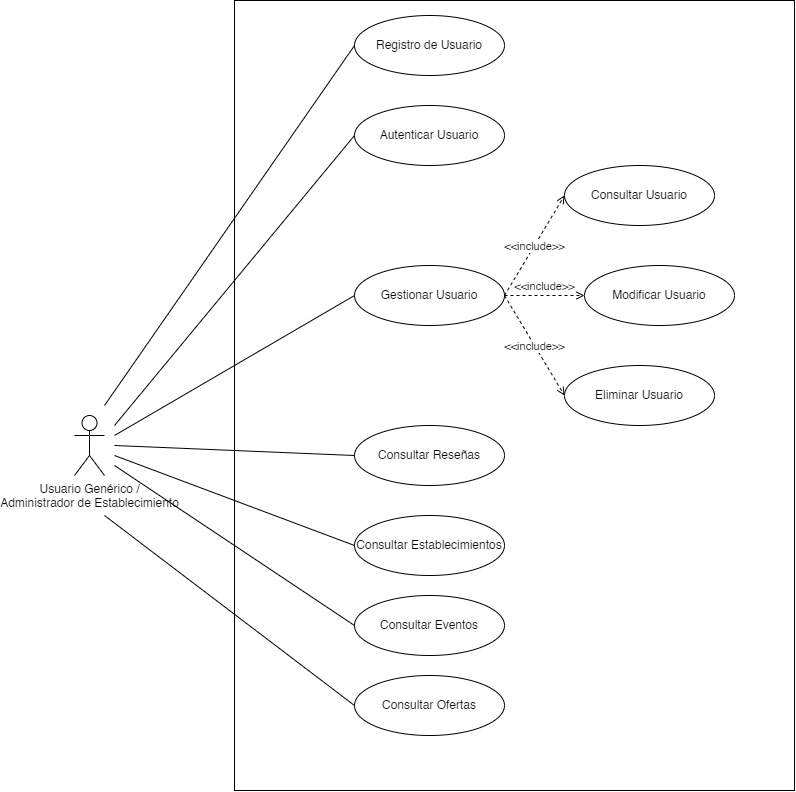
\includegraphics[width=\textwidth]{imagenes/CasoDeUsoComun.jpg}
    \caption{Caso de Uso con Actores Comunes}
    \label{fig:CasoDeUsoComun}
\end{figure}

\clearpage
\begin{figure}[H]
    \centering
    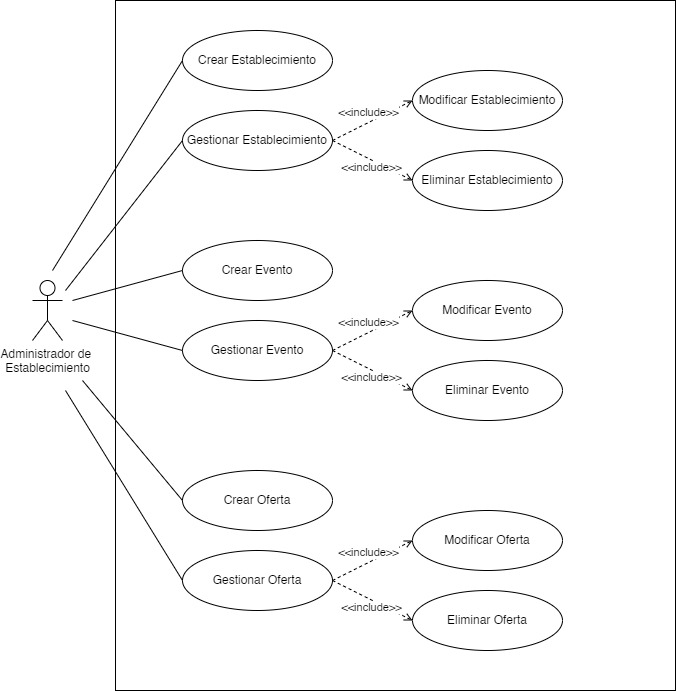
\includegraphics[width=\textwidth]{imagenes/CasoDeUsoAdministrador.jpg}
    \caption{Caso de Uso con Administrador de Establecimiento}
    \label{fig:CasoDeUsoAdministrador}
\end{figure}

\clearpage
\begin{figure}[H]
    \centering
    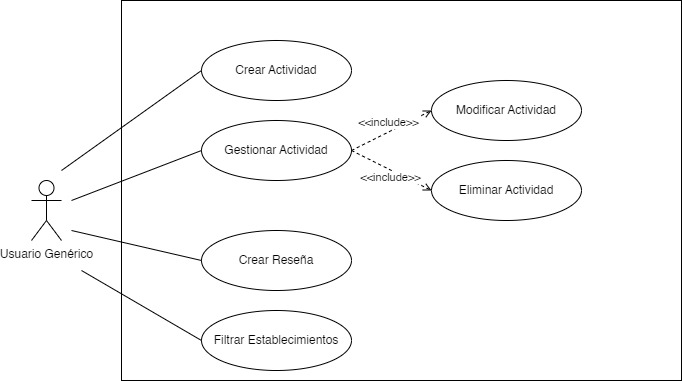
\includegraphics[width=\textwidth]{imagenes/CasoDeUsoUsuario.jpg}
    \caption{Caso de Uso con Usuario Genérico}
    \label{fig:CasoDeUsoUsuario}
\end{figure}


\input{apartados/05_diseño}

\chapter{Implementación}

En esta sección se describen las etapas llevadas a cabo durante el proceso de la implementación del proyecto, los desafíos encontrados y las soluciones adoptadas. También se incluyen ejemplos de código y capturas de pantalla que ilustran el profreso y los resultados obtenidos.

\section{Preparación del Entorno de Desarrollo}

Antes de iniciar la implementación, se realizó la configuración del entorno de desarrollo. Esto incluyó la instalación de todas las dependencias necesarias y la configuración de herramientas de desarrollo mencionadas en el apartado previo, como Visual Studio Code y Postman.


\section{Servidor}

En este apartado, se describe la implementación en el lado del servidor de la aplicación. Se definirá cómo se realizó la estructura del código y su implementación, proporcionando algunos ejemplos para la creación de la API. A continuación, se definirán los pasos seguidos para lograr esta implementación.

\begin{enumerate}
    \item \textbf{Definición de los Endpoints: }Se definieron los endpoints necesarios para gestionar las llamadas relacionadas con la administración de usuarios, establecimientos, eventos, ofertas y reseñas.

    \item \textbf{Implementación del Modelo: } En esta etapa se implementaron las clases necesarias a partir del diagrama UML del capítulo anterior. Estas clases se encargan de gestionar la comunicación con la base de datos y proporcionar una estructura clara y manejable para los datos utilizados en la aplicación.

    \item \textbf{Implementación de Esquemas: } Se implementaron esquemas para la correcta validación de los datos enviados a la API. Para cada entidad se creó un archivo de esquema específico, lo cual organiza mejor el código y asegura que los datos recibidos cumplan con los requisitos esperados. Esta estructuración facilita la gestión y validación de datos, asegurando la integridad y la consistencia.

    \item \textbf{Implementación de los Endpoints: } La implementación de los endpoints se realizó siguiendo una estructura RESTful. Para cada entidad se creó un archivo de servicio y un bluepring, lo cual evita la repetición de definiciones para cada endpoint. Esta estructura modular garantiza una comunicación eficiente y coherente. La organización del código mediante blueprints además facilita la futura escalabilidad de la API.

    \item \textbf{Pruebas en Postman: } Se realizaron diferentes pruebas para comprobar el correcto funcionamiento de todos los endpoints utilizando la herramienta descrita anteriormente, Postman. Se verificaron las llamadas POST para inserciones a la base de datos, las llamadas GET para obtener información, las llamadas PUT para la modificación de datos y las llamadas DELETE para eliminarlos.
\end{enumerate}

\subsection{Servicios}

Las principales peticiones que atiende el servidor son las de creación, consulta, modificación y eliminación de las entidades. Estas operaciones pueden ser realizadas por un usuario genérico o un administrador de establecimiento, dependiendo de las entidades que gestionen.

\subsubsection{Autenticación y Roles de Usuario}

Los usuarios podrán iniciar sesión con su cuenta, lo que generará un token de acceso que servirá en las cabeceras de las peticiones HTTP para identificar al usuario que realiza la solicitud. En algunas operaciones, este token será obligatorio para poder completarse.

Al iniciar sesión, al usuario también se le asignará un "rol". Esto es necesario para mostrar las pantallas correspondientes a su rol cuando el usuario inicie sesión. Esto asegura que cada usuario vea y acceda únicamente a las funcionalidades que le correspondan según su tipo de usuario.

\subsubsection{Wilson Score}

En el diagrama de clases del diseño lógico, cada establecimiento está asociado con reseñas que tienen una calificación entre 0 y 5. Esto da a lugar a una calificación media para cada establecimiento, calculada como la suma de todas las calificaciones divididas por el número total de reseñas del establecimiento. Aunque ordenar los establecimientos por calificación media puede ser útil, es importante considerar la fiabilidad de esta calificación. Por ejemplo, un establecimiento con sólo 2 reseñas y una media de 4.5 no es comparable con otro que tiene 250 reseñas y la misma calificación media. Para abordar este problema, se puede aplicar el método de Wilson Score.

\[ S_w = \frac{1}{{1 + \frac{1}{n} z^2}} \left[ p + \frac{1}{2n} - z\sqrt{\frac{p(1-p)}{n} + \frac{z2}{4n2}} \right] \]

Este método ajusta las calificaciones en función al tamaño de la muestra, proporcionando una estimación más precisa de la calidad del establecimiento. Así se tiene en cuenta tanto la calificación media como la confibialidad de esa calificación en función al número de reseñas. Es una herramienta útil para ordenar los establecimientos de manera más precisa.

\[
    \text{Media del establecimiento} = \frac{\sum \text{calificaciones de reseñas}}{n}
\]

Convertimos la media a una proporción en una escala de 0 a 1:

\[
    p = \frac{\text{Media del establecimiento}}{5}
\]

El valor crítico $z$ para un 95\% de confianza es aproximadamente 1.96.

Calculamos el denominador:

\[
    \text{Denominador} = 1 + \frac{z^2}{n}
\]

Ajustamos la probabilidad en el centro:

\[
    \text{Probabilidad ajustada en el centro} = p + \frac{z^2}{2n}
\]

La desviación estándar ajustada es:

\[
    \text{Desviación estándar ajustada} = \sqrt{\frac{p(1-p) + \frac{z^2}{4n}}{n}}
\]

Finalmente, el límite inferior del Wilson Score se calcula como:

\[
    \text{Límite inferior} = \frac{\text{Probabilidad ajustada en el centro} - z \cdot \text{Desviación estándar ajustada}}{\text{Denominador}}
\]

El Wilson Score se obtiene multiplicando el límite inferior por 5:

\[
    \text{Wilson Score} = \text{Límite inferior} \cdot 5
\]

\clearpage
\begin{algorithm}
    \caption{Cálculo del Wilson Score y ordenamiento de establecimientos}
    \label{alg:wilson_score_ordenamiento}
    \begin{algorithmic}[1]
        \Require{$\text{establecimientos}$}
        \Ensure{Lista de establecimientos ordenados por Wilson Score}

        \Function{wilson\_score}{establecimiento}
        \State \textit{Obtener reseñas del establecimiento}
        \State \textit{Calcular media de calificaciones}
        \State \textit{Convertir media a proporción en escala de 0 a 1}
        \State \textit{Calcular límite inferior del Wilson Score}
        \State \Return Wilson Score
        \EndFunction

        \Function{ordenar\_establecimientos}{establecimientos}
        \State $puntajes \leftarrow []$
        \For{cada $establecimiento$ en $establecimientos$}
        \State $puntaje \leftarrow$ \textit{wilson\_score(establecimiento)}
        \State Añadir $(establecimiento, puntaje)$ a $puntajes$
        \EndFor
        \State Ordenar $puntajes$ por puntaje de forma descendente
        \State $ordenados \leftarrow [puntaje[0] \text{ para } puntaje \text{ en } puntajes]$
        \State \Return $ordenados$
        \EndFunction
    \end{algorithmic}
\end{algorithm}

\subsubsection{Filtrar Establecimientos}

Existen dos filtrados de establecimientos distintos para el backend, uno para personalizar la experiencia de usuario y el otro el filtro usual para poder buscar las preferencias deseadas. El filtro personalizado está basado en las preferencias indicadas por el usuario en su cuenta, es un filtro con una lógica OR es decir que mostrará todos los establecimientos que cumplan con alguna de las preferencias del usuario. Mientras que el otro filtro seguirá una lógica AND en donde se mostrarán únicamente establecimientos con cumplan con todas especificaciones indicadas por el usuario en su seleccionador de ambientes en su página inicial. Ambos filtros estarán también ordenados por el wilson score haciendo que en todo momento al usuario se le muestren las mejores opciones gracias a la valoración de otros usuarios.

\section{Cliente}

\chapter{Pruebas}

Las pruebas en el desarrollo de una aplicación móvil aseguran funcionalidad y confiabilidad, detectando errores para prevenir fallos catastróficos. Validan los requisitos y el diseño desde etapas tempranas, mejorando la precisión y reduciendo costos. Al gestionar sistemáticamente el proceso de pruebas, estas mejoran la calidad del software, haciéndolas indispensables en las prácticas modernas del desarrollo de aplicaciones.\cite{zhu}

Las pruebas realizadas en el proyecto han sido pruebas unitarias en el backend para verificar el correcto funcionamiento de las funciones principales del modelo. Cada entidad realiza las pruebas utilizando un \textit{mock} para simular las peticiones y respuestas de las llamadas a la base de datos.

Para estas pruebas, se utilizó \textit{pytest}, un marco de pruebas en Python que facilita la escritura de casos de pruebas simples y escalables. Pytest además tiene su propio mock gracias a la biblioteca \textit{pytest-mock} que permite la simulación de interacciones con la base de datos. Pytest tiene las siguientes características:

\begin{enumerate}
    \item \textbf{Detección automática de módulos y funciones de prueba}: Pytest encnuentra y ejecuta automaticamente las pruebas definidas en el proyecto sin ninguna configuración adicional.
    \item \textbf{Informes detallados}: Elimina la necesidad de recordar nombres específicos de métodos de aserción, proporcionando informas claros y detallados sobre los fallos.
    \item \textbf{Fixtures modulares}: Permiten gestionar recursos pequeños o parametrizados a largo plazo, facilitando la reutilización y modularidad en las pruebas.
\end{enumerate}

Además de las pruebas unitarias realizadas, la aplicación se encuentra en fase alhpa donde el único usuario que ha interactuado con la aplicación he sido yo. He realizado pruebas desde el frontend para comprobar el correcto funcionamiento de las pantallas y su navegación, y pruebas en Postman para comprobar el envío de información en formato JSON a los diferentes endpoints de la API.

\chapter{Despliegue}



\chapter{Conclusiones y Trabajo Futuro}

\section{Conclusión}

A lo largo de este proyecto, se han abordado desafíos cruciales enfrentados por los jóvenes y turistas que exploran ciudades desconocidas, especialmente aquellos relacionados con la localización de ocio y entretenimiento. La solución propuesta ha demostrado ser una herramienta valiosa, integrando diversas funcionalidades diseñadas para mejorar la eficiencia y la satisfacción de los usuarios en sus actividades sociales y de ocio. Esta plataforma no solo centraliza información relevante y actualizada de eventos y establecimientos sino que también promueve la interacción social y la participación activa de la comunidad.

El desarrollo de \textbf{HangOut} ha contribuido significativamente a resolver la problemática de la fragmentación de la información y la dificultad en la gestión de eventos. Al proporcionar una lista centralizada y personalizada de opciones de ocio, basada en las preferencias del usuario, ha permitido una exploración más intuitiva y un descubrimiento más eficaz de oportunidades de ocio.

El presente Trabajo de Fin de Grado se ha completado satisfactoriamente con el desarrollo de una aplicación móvil diseñada para la búsqueda, gestión y promoción de establecimientos orientados al ocio. Dicha herramienta ha logrado cumplir con los objetivos establecidos al inicio del proyecto, incorporando además diversas funcionalidades que enriquecen la interacción y mejoran la experiencia de los usuarios.

Este proceso ha resultado ser beneficioso tanto a nivel personal como profesional. El diseño y desarrollo de la aplicación desde su inicio me ha brindado la oportunidad de aplicar los conocimientos adquiridos a lo largo del grado. Mediante la implementación de diversas tecnologías y metodologías, he fortalecido mi comprensión en áreas previamente conocidas y he explorado otras que anteriormente había tratado superficialmente.

La selección de las tecnologías discutidas en capítulos anteriores ha ampliado significativamente mi comprensión sobre el desarrollo de aplicaciones, llevándome a alcanzar un nivel de profundidad y práctica que anteriormente no había experimentado. Adicionalmente, la implementación de metodologías de desarrollo ha potenciado mis habilidades en planificación y gestión de proyectos, enseñándome la importancia de adaptarse a los cambios dentro de un ciclo de desarrollo.

En conclusión, este proyecto ha alcanzado exitosamente su objetivo de facilitar la conexión entre usuarios y establecimientos. Adicionalmente, ha reforzado mi capacidad para identificar problemas y diseñar soluciones efectivas, contribuyendo significativamente a mi desarrollo profesional y preparándome de manera óptima para enfrentar los desafíos del mundo real en la ingeniería de software. Además, ha establecido una base sólida para futuras mejoras y desarrollos en este campo.

Cabe destacar que este proyecto es de código abierto y su código fuente se encuentra disponible en el repositorio de GitHub:

\url{https://github.com/AlexColladodev/HangOut.git}.

\noindent Esto permite a otros desarrolladores y entusiastas del software contribuir, mejorar y adaptar la aplicación según sus necesidades.


\section{Trabajo Futuro}

De cara al futuro, se identifican diversas líneas de trabajo mediante las cuales el proyecto podría expandirse, considerando que actualmente el prototipo ha alcanzado el 80\% de su desarrollo. A continuación, se presentan algunas actualizaciones para el trabajo futuro que podrían ser consideradas para completar la aplicación:

\begin{enumerate}
    \item \textbf{Desplegar API: }El despliegue efectivo de la API es esencial para garantizar su accesibilidad y constante funcionamiento. Esta tarea debería priorizarse como una de las primeras mejoras al proyecto, consiste en la configuración de un servidor que sea capaz de gestionar las solicitudes de los usuarios de manera eficiente y segura. Es fundamental que dicho servidor ofrezca escalabilidad para adaptarse al incremento en el número de usuarios, asegurando así el mantenimiento de su rendimiento óptimo.
    \item \textbf{Chat en Tiempo Real: }La implementación de un chat en tiempo real dentro de la aplicación facilitará la comunicación instantánea entre usuarios, eliminando la necesidad de utilizar otras redes sociales para este propósito. Esta funcionalidad no solo mejorará la interacción social, sino que también permitirá organizar actividades de manera más efectiva, adaptando las fechas y horarios a los requerimientos específicos de los usuarios.
    \item \textbf{Galería Común: }La inclusión de una galería común en la aplicación ofrecería a los usuarios un espacio dedicado para compartir fotos y vídeos de sus experiencias en eventos o actividades. Esta funcionalidad facilitaría que todos los usuarios accedan a las fotos de su interés y las descarguen directamente, eliminando la necesidad de solicitarlas a otros participantes.
    \item \textbf{Integración con Google Maps: }Integrar Google Maps permitirá ofrecer funcionalidades avanzadas de localización, como mostrar la ubicación de los establecimientos o especificar la ubicación de donde se realizan las actividades. Esto mejoraría significativamente la usabilidad de la aplicación.
    \item \textbf{Validación de Datos Administrador: }Implementar un sistema de validación robusto para los datos ingresados por los administradores de los establecimientos asegurando que la información proporcionada sea fiable y actualizada.
\end{enumerate}

En resumen, estas mejoras y actualizaciones propuestas están diseñadas para optimizar la experiencia del usuario y continuar el desarrollo del proyecto hacia un producto más completo y funcional.

\bibliographystyle{unsrtnat}
\bibliography{apartados/referencias}



\end{document}
